%%%%%%%%%%%%%%%%%%%%%%%%%%%%%%%%%%%%%%%%%%%%%%%%%%%%%%%%%%%%%%%%%%%%%%%%%%%%%%%%
%2345678901234567890123456789012345678901234567890123456789012345678901234567890
%        1         2         3         4         5         6         7         8

%\documentclass[letterpaper, 10 pt, conference]{ieeeconf}  % Comment this line out
                                                          % if you need a4paper
\documentclass[a4paper, 10pt, conference]{ieeeconf}      % Use this line for a4
                                                          % paper

\IEEEoverridecommandlockouts                              % This command is only
                                                          % needed if you want to
                                                          % use the \thanks command
\overrideIEEEmargins
% See the \addtolength command later in the file to balance the column lengths
% on the last page of the document

\usepackage[utf8]{inputenc}
\usepackage[T1]{fontenc}

\usepackage{xcolor}
\usepackage{cite}

\usepackage{graphicx}

\usepackage{amssymb}

%added
\usepackage{booktabs}% http://ctan.org/pkg/booktabs
\newcommand{\tabitem}{~~\llap{\textendash}~~}
\usepackage{algorithm}
\usepackage{algorithmicx}
\usepackage[noend]{algpseudocode}
\usepackage{multirow}
\usepackage{subfig}
\usepackage{makecell}
\usepackage{balance}
\let\labelindent\relax
\usepackage{enumitem}

\setlist{leftmargin=2.6mm}



% The following packages can be found on http:\\www.ctan.org
%\usepackage{graphics} % for pdf, bitmapped graphics files
%\usepackage{epsfig} % for postscript graphics files
%\usepackage{mathptmx} % assumes new font selection scheme installed
%\usepackage{mathptmx} % assumes new font selection scheme installed
%\usepackage{amsmath} % assumes amsmath package installed
%\usepackage{amssymb}  % assumes amsmath package installed

\title{\LARGE \bf
Performance Prediction for Data-driven Workflows on Apache Spark 
}
%Performance prediction for DAG-based Spark Applications mixing Machine Learning and Analytical Modeling. 

%\author{ \parbox{3 in}{\centering Huibert Kwakernaak*
%         \thanks{*Use the $\backslash$thanks command to put information here}\\
%         Faculty of Electrical Engineering, Mathematics and Computer Science\\
%         University of Twente\\
%         7500 AE Enschede, The Netherlands\\
%         {\tt\small h.kwakernaak@autsubmit.com}}
%         \hspace*{ 0.5 in}
%         \parbox{3 in}{ \centering Pradeep Misra**
%         \thanks{**The footnote marks may be inserted manually}\\
%        Department of Electrical Engineering \\
%         Wright State University\\
%         Dayton, OH 45435, USA\\
%         {\tt\small pmisra@cs.wright.edu}}
%}

\author{Andrea Gulino, Arif Canakoglu, Stefano Ceri and Danilo Ardagna\\Politecnico di Milano, \textit{name.surname@polimi.it}.}




\begin{document}



\maketitle
\thispagestyle{empty}
\pagestyle{empty}


%%%%%%%%%%%%%%%%%%%%%%%%%%%%%%%%%%%%%%%%%%%%%%%%%%%%%%%%%%%%%%%%%%%%%%%%%%%%%%%%
\begin{abstract}

Spark is an in-memory framework for implementing distributed applications of various types.
Predicting the execution time of Spark applications is an important but challenging problem that has been tackled in the past few years by several studies; most of them achieving good prediction accuracy on simple applications (e.g. known ML algorithms or SQL-based applications).
In this work, we consider complex data-driven workflow applications, in which the execution and data flow can be modeled by Directly Acyclic Graphs (DAGs).  Workflows can be made of an arbitrary combination of known tasks, each applying a set of Spark operations to their input data.
By adopting a hybrid approach, combining analytical and machine learning (ML) models, trained on small DAGs, we can predict, with good accuracy, the execution time of unseen workflows of higher complexity and size. \\
We validate our approach through an extensive experimentation on  real-world complex applications, comparing different ML models and choices of feature sets.

%Abstract— Spark is an in-memory cloud computing platformfor implementing distributed applications of various types, suchas  data-driven  scientific  workflows.  Predicting  the  executiontime  of  workflows  is  an  important  but  challenging  problemthat has been tackled in the past few years by several studies.However, those studies either focus on the single task, validatingtheir  models  on  simple  applications  (e.g.  static  applications,known ML algorithms, Spark-SQL-based applications), or justfocus  on  the  makespan  estimation  and  scheduling  problem,without  showing  the  problems  that  arise  when  combining  thetwo things (e.g. XXX when intermediate results will be providedXXX  ).  In  this  paper,  we  tackle  the  problem  of  modelingand  predicting  the  performance  of  DAG-based  applicationsimplemented   on   Spark,   in   which   Directly   Acyclic   Graphs(DAGs)  describe  how  data  flows  through  several  tasks,  eachtransforming the input data through a set of Spark operations.We model the workflow execution time by combining predictionmodels   built   for   each   task   in   the   DAG,   mixing   ML   andanalytical   approaches   in   a   complementary   way.   Predictionmodels  take  into  account  different  features,  such  as  the  inputdata  profiles,  execution  environment  (CPUs  and  memory)  andtask-specific parameters. We apply our methodology to ScQL, acomplex system mapping SQL-like queries to DAG-based SparkApplications  and  we  measure  the  accuracy  of  our  predictionsthrough an extensive experimentation on both artificial and realdatasets.

\end{abstract}

\begin{keywords}
performance prediction, workflow applications, Spark, machine learning
% analytical models. DANILO:  I dropped this, MASCOTS people can possibly think to a Queueing Network and their expectation unattended
\end{keywords}

%%%%%%%%%%%%%%%%%%%%%%%%%%%%%%%%%%%%%%%%%%%%%%%%%%%%%%%%%%%%%%%%%%%%%%%%%%%%%%%%
\section{INTRODUCTION}
In the past decade, we have witnessed an increasing spread of big data applications in several domains, such as business analytics \cite{sun2018big}, social media analysis \cite{ghani2019social}, healthcare \cite{kulkarni2020big}, and natural language processing \cite{Hirschberg261}.
Big data applications are characterized by data-intensive and computationally intensive tasks which are typically implemented on top of  parallel algorithms and distributed computing frameworks. Among such frameworks, Apache Spark has emerged as the de-facto platform for analytical processing, with broad adoption in both industry and academia, due to its simplicity, fault tolerance, and scalability \cite{Hirschberg261}.\\
At the same time, users and enterprises have started moving their big data applications from  traditional local server architectures to cloud computing platforms (e.g. Amazon EC2, Google Cloud, Microsoft Azure\footnote{https://aws.amazon.com, https://cloud.google.com and https://azure. microsoft .com }), which provide configurable environments suiting the needs of big data applications.
These systems usually offer services at the Platform level, where big data  frameworks are already installed, and allow their users to choose among several configurations, e.g. specifying the number of instances in a cluster and their characteristics (CPUs, memory, \ldots).
Each choice might drastically affect  the application execution time and the monetary cost of using the cloud computing service.\\
%Resources allocated to each application should be proportional to its workload, not only to avoid resource wasting but also considering that allocating more resources than necessary might negatively impact on the execution time \cite{li2015sparkbench}.
%\textbf{XXX this is not usual, provide a reference to support this statement XXX: Overcommitting CPU resources leads to CPU contention and adversely impact the execution time, cited paper. }
Predicting the performance of an application is therefore useful for a proper allocation of the available resources, aimed at reducing resource wasting and extra costs.

The problem of performance prediction for big data applications on the cloud has been tackled in several studies. Some  of them rely on traditional techniques, such as analytical models \cite{lundstrom2004, ardagna1, vianna2013} and simulation \cite{Verma2011}.   More recently, machine learning (ML) has been used to predict the performance of large systems \cite{ernest, pan2017hemingway, alipourfard2017cherrypick, ARDAGNA2019}.
The idea is to collect training data offline and use ML models, such as regression, to predict the runtime performance of future executions.
Those studies mainly differ for the chosen set of features (\textit{black-box} vs. \textit{gray-box} approaches), i.e. capturing more or fewer details of the system,  and for the applied ML technique (simple regression vs. more complex ML techniques). In \cite{ARDAGNA2019} authors show how black-box models (specifically Ernest, an approach proposed by Spark inventors \cite{ernest}) fail when applications exhibit irregular patterns and/or when extrapolating on bigger data set sizes.
Despite achieving good results in terms of accuracy, those studies are performed on simple monolithic applications (e.g. static programs, known ML algorithms), which complexity is far from modern data analytics pipelines.
Indeed, nowadays, scientific jobs are rather represented as workflow applications that consist of many complex tasks, with logical or data dependencies, that can be implemented on top of several parallel frameworks \cite{atkinson2017scientific, warr2012scientific, lordan2014servicess}. 
%\textbf{XXX these are old too and I cannot be of help here but I suggest to look at COMPSs papers by Barcelona Computing Center and XXX: we added COMPSs and another paper about scientific workflows}.
%https://books.google.it/books?id=xWoqBAAAQBAJ&lpg=PR3&hl=it&pg=PR3#v=onepage&q&f=false

%Workflows can be implemented on top of platforms such as Apache Airflow (and  KNIME?), which
%Several workflow management platforms are available (e.g. Apache Airflow), and help users schedule and monitor the workflow, or implemented from scratch.
%Each task of a workflow can be then executed as an independent application (each task runs a separate process ... ) or the entire workflow can be mapped to a single application, e.g. being mapped to a single Spark Application. 

%In the last case, the dependencies of each task (incoming edges) represent its input RDDs. This avoids materializing the intermediate results, resulting in more efficient executions.

A workflow application can be  represented by a Directed Acyclic Graph (DAG), i.e. a directed graph with no cycles, in which vertices and their connecting edges are used to represent, respectively,  application tasks and their dependencies. Each task cannot be executed until all its parent tasks have completed their execution and moved their results to their child tasks. Specifically, we target workflow applications implemented on Spark, i.e. workflows in which each task of the workflow applies a set of Spark operations to the task inputs. Moreover, a workflow can be potentially implemented by multiple Spark applications.


%todo: be sure you say that there is a single exit task
A simple way of predicting the execution time of a workflow  could consider the workflow as a monolithic application with known inputs. In this case, a ML model should be trained for each feasible workflow, i.e. for each possible combination of tasks that could appear in the workflow. Besides being a solution that does not scale, the complexity of large workflows could be hardly captured by machine learning. 

% impariamo dai singoli task, svantaggio di non conoscere l'input dei task intermedi

The solution proposed in this paper, instead, builds a separate ML model for each task allowed in a workflow application. The workflow execution time is eventually estimated as a combination of the individual tasks execution time predictions. This type of solution allows training ML models on minimal workflows and uses them to predict the performance of \textit{unseen} workflows of arbitrary complexity.
Moreover, since the input data of intermediate tasks is not known offline, we estimate their characteristics (profiles) by mixing ML and analytical models.


The overall solution is a hybrid approach to estimate the execution time of arbitrary complex workflow applications based on Spark. To the best of our knowledge, no previous work focused on performance prediction for Spark applications presenting this level of complexity and no similar approaches, explicitly tackling the problem of intermediate result estimation, were used for workflow performance prediction.

 %\textbf{XXX I would define your approach  \textit{hybrid} as based on ML and analytical models, and the work would look more original than the number of ML based papers that are popping up today XXX: done}. 
%In this work:
%\begin{itemize}
%    \item  we deal with complex and dynamic configurable workflows, rather than simple and monolithic applications, which are typical benchmarks in previous works on performance prediction for Spark
%    \item we propose a \textit{three-phase} approach for workflow performance prediction: intermediate profile estimation; individual tasks execution times prediction; workflow execution time prediction.
%\item We tackle the problem of estimating the intermediate data profile of a workflow
% \item 
%XXX-- once we do extensive training on simple query - we are able to validate on totally different queries obtaining acceptable error ---XXX it means also small spark dags vs big, unseen dags
%\end{itemize}
%\textbf{XXX say something more on the analytical model role XXX: we added one more line}.

We validate our approach on a real-world complex system, comparing different ML techniques and choices of feature sets (black-box vs. gray-box). Eventually, an extrapolation analysis compares the robustness of different ML models against the variation of the input data size and of the cluster computational power.

This paper is organized as follows: in Section \ref{section:dag_applications} we describe data-driven workflow applications and introduce the real-world system used in our experimental evaluation; in Section  \ref{section:performance_prediction} we describe our three-phase approach for performance prediction, validating the approach in section \ref{section:evaluation}. A discussion of  related literature proposals is reported in Section \ref{section:related_work}. Conclusions are finally drawn in Section \ref{section:conclusions}.

%\textbf{XXX General comment:  Spark is used for big data analyses and ML today/data science.  When you mention scientific workflows the MASCOTS community can think, e.g., to molecules simulations and the like.  Here I would make more explicit the class of applications you consider, which are not classic scientific applications as above.  There is a mismatch otherwise also in the way you model the DAG which is data-oriented (e.g., to simulate molecules you don't need probably to characterize the data model (relational/semistructured, etc., Sect 3 XXX: DISCUSS} 


\section{Data-driven Workflow Applications}
\label{section:dag_applications}


A data-driven workflow application can be represented as a Directly Acyclyc Graph (DAG), i.e. a directed graph with no cycles. Each vertex in this DAG represents a task, while edges represent the data and control dependencies between tasks.  A task is executed only when all its input data have been computed, i.e. when all parent tasks have completed their execution.
%$G=(V,E,L)$
Formally, a DAG representing a workflow application can be described as a tuple $G=(V,E)$, where $V$ is the set of vertices (tasks), $E$ the set of directed edges (dependencies) s.t. $E\subseteq V^2$.
We call \textit{entry task} (\textit{exit task}) a task with no incoming (outgoing) edges. For simplicity, we assume that workflows have a unique exit task.  While entry tasks represent the reading of the workflow input data, the exit task stores back its final result. We further assume that each task produces a single output, which can be the input to multiple child tasks (through multiple edges).
%, and $L$ a labelling $L: E \to \mathbb{N}$, assigning each edge $e=(v,w)\in E$ a label, uniquely identifying the output data of task $v$.
%The aciclicity is given by assuming that the transitive closure $E^+$ of the relation $E$ is irreflexive; i.e. $(v, v) \not \in E ^+ ,\ \forall v \in V$. An edge  $e=(v,w)\in E$ is called \textit{outgoing edge} of vertex $v$ and \textit{incoming edge} of vertex $w$.

%, i.e.: 
%$$\nexists \ e=(v,w), e'=(v,w') \in E \ | \ w\not=w' \wedge L(e)\not=L(e') $$
%meaning that the output data of a task is unique but can be dispatched to multiple child tasks.



%Moreover we define the set of \textit{predecessors} of a task $v \in V$ as $pred(v) =\{ w | (w,v) \in E \} $ and the set of its \textit{successors} as $succ(v) =\{ w | (v,w) \in E \}$.
%\textbf{XXX In the introduction you discussed the possibility to have mutiple exit task: This open the problem to predict performance of a path in the DAG or the average execution time of the full DAGs according to the probability distributiosn of its execution path.  The simple approach is remove in the intro mutiple exit tasks and here state explicitely that we focus on single exit task, i.e. we have a single execution path in the DAG XXX: we assumed that our DAGs have only one exit task in the intro + previous paragraph.} 
%\begin{figure}
%  \centering
%  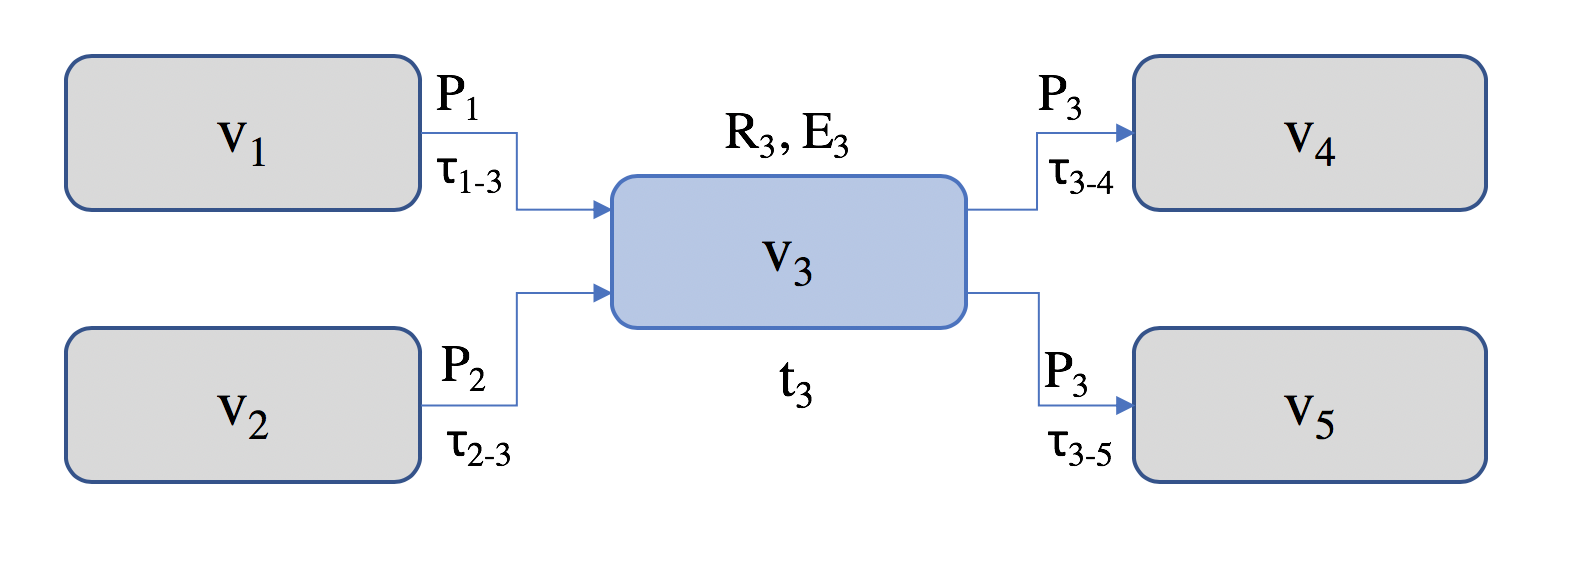
\includegraphics[width=0.48\textwidth]{sources/task.png}
%  \caption{Characterization of a generic task of the DAG ($v_3$). 
  %According to our definition $P_{3\rightarrow4}=P_{3\rightarrow5}$
%  }
%\label{fig:operator}
%\end{figure}


\noindent Moreover, we characterized each task defining:
\begin{itemize}
    
    %\item \textit{Data Profile}:  $P_{i\rightarrow j} = \{p^{i\rightarrow j}_1, p^{i\rightarrow j}_2, \ldots,p^{i\rightarrow j}_{|P_{i\rightarrow j}|}\}$, associated to each edge $(i,j)\in E$, represents the profile, i.e. a set of features providing a quantitative description, of the output data generated by task $v_i$ and delivered to task $j$. We also define the set of input profiles  of a task $\Pi^{in}_i = \{ P_{j\rightarrow i} | (j,i) \in E\}$ and its dual  $\Pi^{out}_i = \{ P_{i\rightarrow j} | (i,k) \in E\}$, that will contain only a single profile ($|\Pi^{out}_i| \leq 1$), given that the output data of each task is assumed to be unique. The set of features in $P_{i\rightarrow j}$ follows the same schema for any $i$ and $j$.
    \item \textit{Output Profile}: a set of features quantitatively describing its result.
    %$P_{i} = \{p^{i}_1, p^{i}_2, \ldots,p^{i}_{|P_{i}|}\}$, associated to each task $v_i\in V$, represents the profile, i.e. a set of features providing a quantitative description, of the output data generated by task $v_i$ and delivered to all its successors $succ(v_i)$. We also define the set of input profiles  of a task $\Pi_i^{in} = \{ P_{j} | v_j \in pred(v_i)\}$. For every task in the DAG, output profiles are described by the same set of features. 
    %\textbf{XXX Not clear here what you mean, you consider the same set of features? XXX: sentence is changed. }
    
    \item \textit{Task Arguments}: any input  parameter given to the task, in addition to the input data produced by its parent tasks. Examples can be strings, flags or other options that might change the behaviour of the task.
    %$R_{i} = \{r^i_1, r^i_2, \cdots, r^i_{|R_{i}|} \} $, associated to each task $i$, denotes the set of specific parameters for task $v_i$. Examples can be selectivity, filter option and so on ... not binning (see next point). The set of features in $R_i$ follows the same schema for any $i$.
    \item  \textit{Environment Parameters}: %($E_{i} = \{e^i_1, e^i_2, \cdots, e^i_{|E_{i}|} \} $), associated to each task $v_i$, denotes the
    a set of features describing the execution environment in which the task will run. Examples are the number of cores and amount of memory of a cluster.
    %task  $v_i$ (e.g. number of CPUs, memory, partitions). In this set we include all those parameters that do not affect the result of the task, but just its performance (e.g. binning). The set of features in $E_i$ follows the same schema for any $i$.
    \item \textit{Execution Time}: 
    %($t_i$), which applies to each task of the workflow. It corresponds to the 
    time required for processing the input data and produce the task result. %(unique) output $L(v_i)$. As later discussed, this time depends on the input data, task and environment parameters. 
    %\item \textit{Transfer Time} ($\tau_{i\rightarrow j}$), associated to each edge $(i,j)\in E$, represents the time required for moving the output of a task to its successors. An example might be network transfer  data time.
\end{itemize}


%\color{red}
%We should discuss what is a task in practice in a workflow based on Spark: e.g. a task encapsulates one or more Spark Jobs and the entire workflow is a single spark application, or each task could be a single Spark Application.
%\color{black}


%\color{black}
%The modeling of the workflow as described above is independent of the input data types, which can be relational records, semi-structured documents or plain text items.
%\color{black}

\subsection{Target Application}
\label{subsec:scql}
\begin{figure}
  \centering
  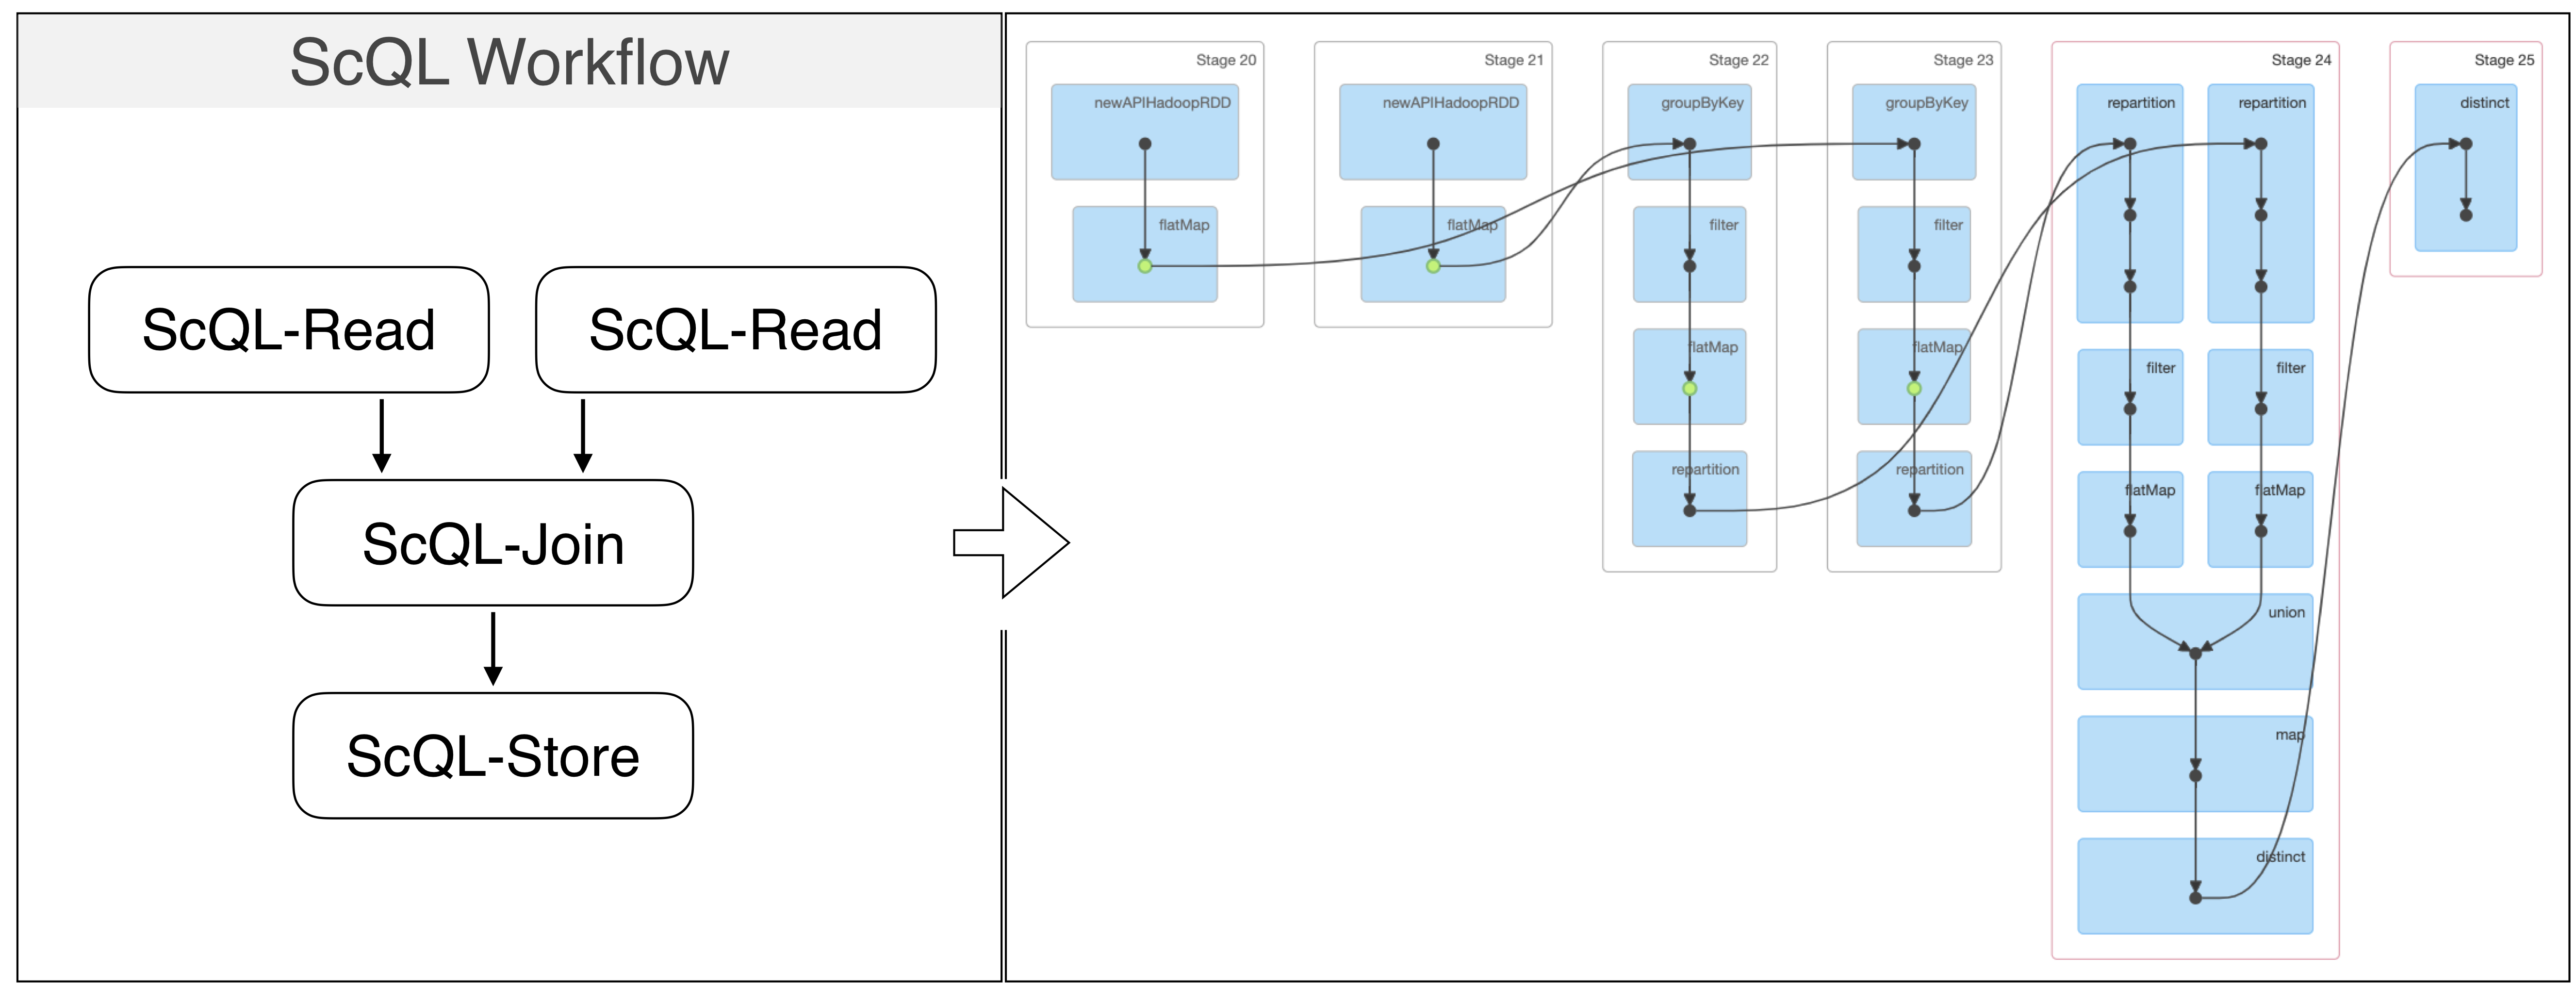
\includegraphics[width=0.5\textwidth]{sources/scql_mapping.png}
  \caption{A ScQL Workflow is mapped to Spark DAG Application.}.
\label{fig:scql-dag}
\end{figure}

\noindent 
For our experimental evaluation, we chose a real-world cloud system that maps complex workflows to Spark applications.  This system implements a SQL-like language for interval data called ScQL \cite{ScQL,gmql}.

Like for other query languages relying on relational algebra, a ScQL query can be easily mapped to a workflow, in which each task represents a query operator.
A simplified version of a ScQL query is the following:
\begin{verbatim}
    DS1 = READ() dataset_1;
    DS1 = READ() dataset_2;
    RES = JOIN(dist<100) DS1 DS2; 
    STORE RES;
\end{verbatim}
Once a query is submitted, the ScQL processing system translates the query into a ScQL-Workflow, similar to the one depicted on the left side of Fig. \ref{fig:scql-dag}.
Each task of this workflow applies a set of Spark operations on input data to implement the semantics of the corresponding ScQL operator. In this specific example, the entire workflow corresponds to a single Spark application, which DAG structure is depicted on the right side of Fig. \ref{fig:scql-dag}.

In the ScQL Data Model, an interval-dataset $D$ is made of several files (which in memory are called \textit{samples}). Each entry in a file represents an interval, by means of its start and stop values.\\
Although ScQL includes several operators, in our experimental evaluation we will only mention two of its most complex and peculiar operators, namely ScQL-Map and ScQL-Join, that are here briefly described: 
\begin{itemize}
    \item \textbf{ScQL Map}: given two input datasets,  namely a \textit{reference} and an \textit{experiment} dataset, this operator computes, for each interval in the reference dataset, aggregates on the overlapping experiment intervals. 
    \item \textbf{ScQL Join}: given two input datasets, namely a \textit{reference} and an \textit{experiment} dataset, this operator computes, for each couple of reference-experiment files, the couples of overlapping reference-experiment intervals.  A \texttt{distance} parameter (dist) can be provided to match also experiment intervals which are at a maximum distance from a reference interval. 
\end{itemize}
Lastly, we mention a partitioning technique called \textit{interval-binning} \cite{binning}. The \textit{bin-size} parameter determines the amount of intervals that end up in the same partition. Depending on this parameter, some intervals of the initial dataset might be replicated in several partitions.

%We don't consider metadata computation, that is performed in a short period before query execution and just filters the initial inputs. Therefore we deal only with an equivalent workflow DAG made of only operations which are applied to observations.

\section{Workflow Performance Prediction}
\label{section:performance_prediction}
Our \textit{three-phase} solution for predicting the execution time of a workflow application performs
%, in order,  
the following three steps:
%\begin{itemize}
%    \item a \textbf{DAG}: as previously described, in which, for each task $v_i$, the sets $R_i$ (task parameters) and $E_i$ (environment parameters) are already set.
%   \item all \textbf{input profiles}: data profiles of the workflow input datasets, i.e. $P_i$ for each task $v_i$ that is an entry task. 
%\end{itemize}
\begin{enumerate}
    \item \textbf{Intermediate profile estimation}: for each task in the workflow, its output profile is estimated. This implies that, at the end of this phase, the input data profile of every task in the workflow will be available.  This phase is detailed in Section \ref{section:intermediate_input}.
     %\item (maybe here there is a phase in which we set, for each task $v_i$, the actual number of resources that can be used (i.e. we set $E_i$), depending on the number of other tasks which can be run in parallel with $v_i$. 
    \item \textbf{Task execution time prediction}: for each task of the workflow, its execution time is predicted. This is discussed in section \ref{section:task_modeling}.
     \item \textbf{Workflow execution time prediction}: the overall execution time is computed by combining the predictions of the individual tasks execution times. Generally, the workflow execution time depends on the underlying engine and its scheduling algorithm. In this work we target workflows that are mapped to Spark applications. By assuming that: i) every task of a workflow is executed within the same Spark context; ii) every workflow task corresponds to a number of Spark tasks that is greater or equal to the number of available cores (in other words,  assuming that each workflow task will keep busy all the available cores) then we can reasonably approximate the workflow  execution time as the sum of the individual tasks execution times. The validity of these assumptions is proven by our experimental results (see Section \ref{section:evaluation}).
\end{enumerate}

%The makespan of a workflow is the time required to execute all the tasks in a workflow. In general, the makespan is lower bounded by a minimum time given by the longest path from any entry task to any exit task (critical path), and upper bounded by the time spent to execute all the tasks sequentially (including transfer costs). \textbf{XXX If you have mulitple exit tasks is still critical path a lower bound for excetuion ? XXX: resolved}

%The  makespan is tightly dependent on the topology of the workflow and on the scheduling algorithm used by the WMSM, that, given that the scheduling problem is NP-complete, applies heuristics to produce minimal cost schedules.

%Although using ML techniques, might be a good way to estimate the makespan of a workflow on a generic workflow system, in this paper we focus on workflows built on top of Spark. Assuming that :

%$$ \sum_{i\in V} t_i + \sum_{(i,j) \in E} \tau_{i\rightarrow j}$$
%\textbf{XXX so data transfer are zero? I would state at the beginning and I would not add complexity to the model.  Moreveor, do you assume that all tasks are sequential? XXX: DISCUSS}



%\begin{figure}
%  \centering
%  \includegraphics[width=0.38\textwidth]{sources/perf-es%timation-module.png}
%  \caption{Steps performed by the performance estimation %module to produce an estimation of the workflow %execution time, given the workflow DAG and the input %profiles.}.
%\label{fig:module}
%\end{figure}



\subsection{Task execution time prediction}
\label{section:task_modeling}
%In this section we describe how the execution time of a task can be predicted by machine learning. 
%However, the approach described in this section is used also to perform output-data profile estimation as discussed in section \ref{section:intermediate_input}. 
The goal of task execution time  prediction is to build, for each different type of task that can be present in a workflow, a machine learning model that, with \textit{adequate} accuracy, is able to predict the task execution time.
%\textbf{XXX (output data size) XXX: we were referring to this section not to output estimation; we made it clear.}
A ML model is trained on a set of features characterizing the task, such as a quantitative description of its input data, its arguments, and features describing the execution environment, with the objective of predicting its execution time. \\
%In this section, we give importance to the choice  of features, proposing a categorization that depends on the knowledge of the application, its data model and the execution environment, and on the complexity of the defined features.
%The choice of features to be included in the feature set is crucial for the accuracy of the generated models. The more the feature set resembles the set of features composing the (unknown) underlying model, the higher will be the model accuracy. 
Identifying and extracting a complete set of features is hard to achieve in this context. First of all, the knowledge on the application and on the execution environment might be limited; secondly, extracting some features might be non-trivial and time-consuming, hence not convenient.  Third, a super-set of features usually leads to overfitting.

State-of-the-art ML solutions for performance prediction are mostly based on simple feature sets that provide an high-level description of the input data and of the execution environment. 
These are usually called \textit{black-box} features, e.g. the input size and the number of cores can be considered a complete set of black-box features for the performance prediction of a generic parallel application.
Although it has been proven that black-box features can be powerful enough to get good prediction accuracy (e.g. in Ernest \cite{ernest}), choosing a simple feature set might become limiting when trying to describe the performance of  complex workflows.
%of more complex applications; e.g. workflow applications.

In this work, we considered different feature sets, showing how different choices can impact the prediction accuracy of the produced models. Without constraining the choice of features, we propose a categorization of the possible feature sets. The first distinction we make is between: 
\begin{itemize}
    \item \textbf{Black-box} features, that do not require detailed knowledge on the application, data model and execution environment.
    \item \textbf{Gray-box} features, that extend black-box features with application, data-model  and environment-specific features. We assume that gray-box feature sets include also black-box features.
\end{itemize}
Orthogonality to the previous distinction, we discriminate among:
\begin{itemize}
    \item \textbf{Basic features}, organized into:
    \begin{itemize}
        \item \textbf{Input Data Profiles}: features quantitatively describing the input data of a task (e.g. data size, number of files, number or entries ...).
        \item \textbf{Task Arguments}: any input parameter given to the task.
        %a set of features representing the arguments of the task. For a task $v_i$, it is equivalent to the set $R_i$ mentioned in  section \ref{section:dag_applications}.
        \item \textbf{Execution Environment}: a set of features describing the environment in which the task is executed, e.g. number of cores and amount of memory, or more advanced features characterizing the Spark environment.
    \end{itemize}
    \item \textbf{Composite features}. Even though several machine learning methods are able to capture non-linear dependencies on the features, it is sometimes "helpful" to include non-linear combinations of some basic features in the final feature set. For example, Ernest \cite{ernest} 
    %\textbf{XXX Ernest cite XXX: DONE}
    introduced the logarithm of the number of cores, which encodes the cost of reducing operations in parallel frameworks, and the ratio between data size and number of cores, which approximates the time spent in parallel processing. 
    %\textbf{XXX Add also the discussion on data size/ number of cores since otherwise it is not clear that you perform combinations below XXX: DONE}.
    We define composite features as linear or non-linear combinations of basic features.
\end{itemize}



\begin{table}
\caption{Feature-set categorization}


\centering
\label{tab:feature-sets}

\resizebox{1\columnwidth}{!}{
\begin{tabular}{|c|c|c|}
    \hline
 & Basic & Full \\
    \hline
    \multirow{3}{*}{Black-box} & Input Data (BBI) &  BBI $\cup$ BBT $\cup$ BBT \\ 
    &Task Parameters (BBT) &  Composite Features (BBC) \\
     &Execution Environment (BBE)  &   \\
     \hline
    \multirow{3}{*}{Gray-box} & Input Data (GBI) & GBI $\cup$ GBT $\cup$ GBT \\ 
    &Task Arguments (GBT) &  Composite Features (GBC) \\
     &Execution Environment (GBE)  &   \\
    \hline
\end{tabular}
}

\iffalse
\centering
\caption{Example of features in the four categories}
\label{tab:feature-sets-instance}

\resizebox{1\columnwidth}{!}{
\begin{tabular}{|c|c|c|}
    \hline
 & Basic & Full \\
    \hline
    \multirow{3}{*}{Black-box} & BBI = input-size, num-files &  BBI $\cup$ BBT $\cup$ BBT \\ 
    &BBT = arg1, arg2 $\cdots$ &  BBC = input-size/cores, log(cores) \\
     &BBE = memory, cores  &   \\
     \hline
    \multirow{3}{*}{Gray-box} & GBI = BBI + interval-length & GBI $\cup$ GBT $\cup$ GBT \\ 
    &GBT = distance & GBC = BBC + input-size/num-tasks \\
     &GBE = BBE + num-tasks  &   \\
    \hline
\end{tabular}
}
\fi
\end{table}
\noindent Given the aforementioned distinctions, we organize the possible feature sets in four categories, summarized in Table~\ref{tab:feature-sets}: basic black-box features (\textbf{BB-Basic}); basic and composite black-box features (\textbf{BB-Full}); basic gray-box features (\textbf{GB-Basic}); basic and composite gray-box features (\textbf{GB-Full}).

%In Table \ref{tab:feature sets-instance}, we provide an instance for each of these four categories. 

According to the proposed categorization, Ernest, i.e. the state-of-the-art for Spark application performance prediction, uses a black-box full (BB-Full) feature set. In the experimental evaluation, our choice of features for the BB-Full feature set included all the Ernest features and will be considered a baseline to evaluate the benefits of our approach.

For each category, we defined a set of candidate features on which we applied Sequential Forward Selection (SFS) \cite{kudo2000comparison} to remove non-relevant ones.
%What we denote as feature set should be considered an initial set of features which may also include non-relevant features. A proper feature-selection algorithm should be used to remove any non-relevant feature from the set.

% ARIF: we can change the reference and move this sentence to section intermediate_input

%In \ref{section:intermediate_input}, we use the same feature set distinction for predicting the output data profile of a task, excluding execution environment features.

\subsection{Model Techniques}
%\textbf{XXX This section is generic, focus and state what you used XXX: we removed unused techniques and anticipated some results}

In the previous works, Venkararaman et al. \cite{ernest} (Ernest's authors)  and Maros et al.\cite{ARDAGNA2019} have applied ML to estimate the execution of simple Spark applications. While Ernest is based on linear regression, with coefficients estimation based on non-negative least squares (NNLS), in Maros et al. authors took into account more complex ML techniques such as Decision Tree and Random Forest.\\
%This is a variant of the least squares algorithm with the added restriction that coefficients must be non-negative. This restriction ensures that each term provides a non-negative contribution to the overall execution time, preventing estimation of negative execution times.
%In \cite{ARDAGNA2019}, four classic ML techniques have been compared, including L1-regularized linear regression (LASSO), neural networks, decision trees, and random forest. \\
In Section \ref{section:evaluation} we compare the performance of three suitable ML techniques: (i) Linear regression (LR), which produces models that can be easily interpreted, but hardly captures complex interactions between features, (ii) Decision Trees (DT) and (iii) Random Forest (RF), having the ability to capture non-linear relationships, still allowing a good interpretability of the model.
    %\item Neural Networks (NN) can capture non-trivial interactions among the input features albeit less interpretable.

Given a target task type, for which we want to predict the execution time, the training set provided to the chosen machine learning technique is made of several executions of that task. 
As proven in the experimental section, depending on the feature set and on the model technique, it might not be necessary to run on big inputs and extremely powerful environments. Even running small executions on medium-size clusters can still produce prediction models with good prediction error on larger inputs and clusters.
%In the experimental section we analyze the performance of different model techniques on different feature sets, showing the advantages and drawbacks of using one model w.r.t. another and testing the model robustness against the variation of some relevant features  (e.g. data size and number of cores). 
%Specifically, we show how RF and DT have higher accuracy and robustness w.r.t. LR. 





%\subsection{Training and Test Sets}

%ARDAGNA2019\\
%\color{black}
%To learn and evaluate the ML models, data coming from the experiments are split into training and test sets. The former is used to learn the model, whereas the latter is used to evaluate its accuracy. Since hyper-parameters tuning is performed for each ML technique (see Section IV-D), a sub- set of the training data is used for cross-validation to reduce over-fitting. For each workload, we evaluate the accuracy of the prediction models in terms of core interpolation and data size extrapolation capabilities, acknowledging the fact that the data available for learning the models (training set) might have been obtained via experiments on setups different from the one for which the prediction is needed (test set). Figure 1 and Table II summarize the scenarios considered.
%In the core interpolation scenarios, we consider runs with the same dataset size (reported in Table II) and verify the capabilities of the trained models of interpolating the number of cores. Figure 1 shows the various scenarios (y-axis) of core interpolation built for each workload based on different splits of the data into training and test sets: in each row (case number), blue boxes represent configurations for which the data were used as part of the training set (and cross- validation) and red crosses indicate configurations used as part of the test set10. We designed scenarios such that larger case numbers are associated with harder predictions, as their training data include samples from a smaller range of experiments w.r.t. the number of cores. In the data size extrapolation scenarios, we put the runs with the largest dataset size (spanning across all available cores configurations) in the test set while the runs with the other dataset sizes in the training data, as shown in the two rightmost columns of Table II. Moreover, training sets are further reduced by removing runs according to the same schema presented for core interpolation. By doing so, in these experiments we evaluate at the same time the core interpolation and the data size extrapolation capabilities. In other words, these experiments differ from the core interpolation scenarios because: (i) the dataset sizes in training and test sets are no longer the same, (ii) in the test set we also include observations where the number of cores is the same as in some observations of the training set (but again with different dataset sizes).
%\color{black}


\color{black}
\subsection{Predicting intermediate input features}
%\begin{algorithm}[t]
\begin{algorithmic}
\Procedure{profileEstimation}{$v_i$}
  \State\textit{Input:} $v_i \in V$
  \State\textit{Output:} the estimated profile $P_{i}$.\\

  
	\If{ $v_i$ is an entry task}
        	\State $P_{i}$ = load offline-computed profile
    \Else
           \State   $\Pi^{in}_i  = \emptyset$
           	\For {each $v_k \in pred(v_i)$ } 
           	    \State $P_{k} = ProfileEstimation(v_k)$
           	    \State  $\Pi^{in}_i   = \Pi^{in}_i  \cup P_{k}$
           	\EndFor
           	
           	\State $P_{i} = \emptyset$
           	\For{each feature $p$ of the profile schema}%$i \in \{1,\cdots,|P|\}$
           	    \State $P_{i}$ = $P_{i} \cup  predict(i, p, \Pi^{in}_i, R_i)$
            \EndFor
    \EndIf
\EndProcedure
\end{algorithmic}
\end{algorithm}
\label{section:intermediate_input}
In order to perform the task execution time prediction step, all the input features, including the input data profiles, must be available offline. However, this does not hold for intermediate tasks, which input data have not been computed yet. To address this problem, we perform, as the first step, an estimation of all such data profiles.\\
We assume that entry tasks import data which have already been profiled.
%, thus not impacting neither on the run-time nor on the performance-prediction time. 
This assumption is in general acceptable, since application users typically download a limited number of datasets which are then re-used for several workflow runs and can therefore be profiled once for all.
%\begin{itemize}
%    \item the application users typically download a limited number of datatasets which are re-used for multiple workflows, or, at least, several runs of the same workflow (e.g. when fixing / improving the workflow). The data could be profiled once imported, and the profile would be available for multiple executions.
    %\item The profiling task is usually simpler and less time consuming w.r.t the workflow that uses it; i.e. the profiling time is neglectable w.r.t. to the workflow execution time.
%    \item  even this initial profiling could be performed approximately in a short time. E.g., Haas et al.\cite{haas1995sampling} base their estimation on data samples, empirically comparing various estimators from literature. 
    %This way of profiling data is less time consuming and could be also a good runtime solution in case offline profiling resulted unfeasible. 
%    However, a low accuracy of this estimation would negatively affect the quality of performance prediction.
%\end{itemize}

 The goal is to estimate, for every task $v_i \in V$, which is not the exit task, its output profile $P_i$.
 Specifically, an estimation model should be built for each feature in $P_i$. (e.g. data size, number of entries, etc.). \\
 Similarly to the execution time prediction, the feature set used for this type of estimation includes: i) the input profiles of task $v_i$, ii) the task arguments.  Moreover, the same feature set  categorization proposed in section \ref{section:task_modeling} has been applied, reasonably excluding any environment-related feature.
 
\noindent Each feature in $P_i$ can be estimated:
\begin{itemize}
    \item \textbf{Analytically}: there is a known combination of features of the chosen feature set which allows to exactly compute the output feature.
    \item \textbf{Heuristically}: the exact formula for computing the output feature is unknown or there is not enough information to compute it; in this case,  heuristics on the available feature set can be defined.
    \item by \textbf{Machine Learning}: applying ML to estimate the output feature, similarly to what was has been said  for task execution time prediction.
\end{itemize}
The intermediate profile estimation phase estimates each task output profile, starting from entry nodes, which input data profile was computed offline (previous assumption), up to the exit node.\\
In the experimental section (\ref{section:evaluation}) we compare different ways of predicting the output profiles, showing the advantage of using heuristics/analytical models w.r.t. ML. 
Even though heuristics and analytical models require more knowledge on the application, they are able to guarantee lower prediction error.
Analytical and heuristic-based based estimations for ScQL (GMQL) are described in \cite{binning}.

%\noindent For convenience, we define the procedure:
%\begin{equation}
%\label{eq:predict}
%predict(i, p, \Pi_i^{in}, R_i)
%\end{equation}

%\noindent which, given a task $v_i$, its input profiles $\Pi_i^{in}$ and task parameters $R_i$, returns the estimated output profile $P_i$.
%Finally, as mentioned in \ref{subsec:pipeline}, before predicting tasks' execution time, all the input profiles are  estimated by calling the recursive procedure \textproc{profileEstimation}(e), starting from $e$, which is the exit task of the DAG.\\
%\color{black}

%\color{black}
%\textbf{XXX Here it is not clear what you do in concrete. The problem its clear but not its solution XXX: spoiler on the experimental section}

%\subsection{Data Collection}
%\label{subsec:data-collection}

%Each execution should be described by:
%\begin{itemize}
%    \item All the features contained in the selected feature set
%    \item The execution time
%    \item Features describing the output data, coherently with the features chosen to describe the input data. These features are required if the output estimation is performed by machine learning (see section \ref{section:intermediate_input}).
%\end{itemize}
%Although some machine learning methods are quite robust to noise, it is advised to use a clean execution environment entirely dedicated to training data collection. To further eliminate noise, the task should be the only task in the DAG (unless some entry task or exit task is necessary).


%Notes on Spark scheduling:

%In a Spark job, multiple independent stages (e.g., stage 0 and stage 1 to 14 in App 2 as shown in Fig. 1(b)) can be executed simultaneously. Spark standalone mode provides the following two schedulers to manage the execution of multiple stages.
%- FIFO: (first-in-first-out) assigns the resources based on the stage submission order. When all the tasks in a stage are served, FIFO starts to consider the resource assignment for the next stage.
%- FAIR: allows the system to assign different (fixed) weights to jobs and group them into pools based on their weights [3]. However, we find that neither of them can work well with complex data flows. First, the performance of FIFO heavily depends on the order of stage submission which is often decided by user’s application codes. A slight difference in the user codes with the same function can yield a significant difference in the performance1. In addition, while serializing the execution of all the stages, FIFO does not use the knowl- edge of the DAG structure to determine the execution order of the stages. This can certainly cause delays at the stages that need the input from other stages. Second, while FAIR allows parallel execution of multiple stages, it does not carefully consider the DAG structure, either. Moreover, the resources are equally distributed among the stages without considering their individual workload. As a result, FAIR may mitigate the performance issue in FIFO under some cases, but under other cases, as we show in Section II-D, FAIR could perform even worse than FIFO.


%Layered model for estimating worflow makespan:


%\color{black}
%A model for estimating the makespan of a scientific workflow takes into account the workflow structure and divides tasks into levels based on the dependencies between them, so so that tasks assigned to each level are independent to each other. Then, for each level, its execution time (which is equal to the time required for the execution of the tasks in that level) can be calculated considering the overall runtime of the tasks of that level (that is the sum of the individual tasks runtime). The assignment in levels can be done using either a top-down or a  bottom-up approach that assigns a level to each task by taking into account the level of its predecessors or successors respectively. Once the assignment has taken place, a level-based estimation model takes into account level characteristics to provide an overall performance estimate for the workflow.
%\cite{pietri2014performance}

%control flow / data flow

%During execution, we assume that the system schedules as many resources as required to run a single vertex. As such, the vertices are executed sequentially. This is orthog- onal to the fact that within a vertex, execution is performed in a both pipelined and partitioned parallelism manner.
%\cite{gounaris2017dynamic}


%A New Makespan Estimation Model for Scientific Workflows on Heterogeneous Processing Systems

%https://ieeexplore.ieee.org/abstract/document/8411037


%The execution machine is exclusively dedicated to the data flow execution. I.e., we assume that an execution machine executes only one data flow and the execution of the next flow can be started only after the completion of the previous flow. So, the available machine executes tasks and stores data for a single data flow at a time.
%gao2017autopath
%\cite{gao2017autopath}



\section{Experimental Evaluation}
\label{section:evaluation}
We applied the proposed performance prediction model to ScQL DAGs, introduced in \ref{subsec:scql}, focusing on two of its most complex and peculiar operators. In this section we:
\begin{itemize}
    \item describe the experimental setup (\ref{subsec:exp-setup}), the evaluation metric and how hyper-parameter tuning was performed (\ref{subsec:error-hyper})
    \item assess the accuracy of task execution time prediction for different choices of feature sets, different ML techniques and execution environment configurations (\ref{subsec:results-task}).
    \item assess the accuracy of output profile estimation, either using analytical models/heuristics, and ML (\ref{subsec:results-profile}).
    \item measure the error in predicting the workflow execution time, comparing  gray-box models to the state of the art black-box based (\ref{subsec:results-workflow}) and validating on workflows that were much more complex than the workflows used for collecting training data.
    \item present an extrapolation analysis, in which we compare the \textit{robustness}  of different ML models against the increase of the input data size and of the cluster computational power (\ref{subsec:extrapolation}). Specifically, we prove that models trained on small input data (number of cores) are good at predicting execution with larger input data (higher number of cores). This is particularly beneficial, given the nature of big data analyses, in which the size of processed data gets bigger and bigger, as well as the computational resources required for processing.
\end{itemize}


\color{black}
%The accuracy of models using basic and composite black-box features is comparable to the accuracy provided by the state of the art (\textit{Ernest}).
\color{black}

%\begin{itemize}
%\item Application 
%\item Application profiling and training set collection:  environments, number of runs, etc.
%\item Setup of hyper parameters and MAPE
%\item Description of the analysis:  single task estimate and DAG, which DAG did you consider?  Introduce their representation, introduce extrapolation analysis on data size and number of available cores 
%\item results in single tasks
%\item results on data output prediction accuracy
%\item results on DAG accuracy
%\item Discussion on extrapolation analysis
%\item. Whenever is possible comparison with Ernest 
%\end{itemize}
%Moreover, we used single machine (SM) provided by the CINECA computing centre, with 72vCores, 213GB RAM, Spark 2.3.2, on Ubuntu 18.04.4 LTS.
%\textbf{XXX Results here are all based on AWS?  Did you drop your internal node?  Below you mention single node:  stress this cover a continuum where you run you application on a large multi-core node and distributed cluster to validate your approach  XXX: DONE, WE REMOVED ANY MENTION TO SINGLE MACHINE EXECUTION}

\subsection{Experimental setup}
\label{subsec:exp-setup}
\color{black}All the experiments in this section were run on Amazon AWS (EMR service) \color{black}choosing a variable number of \texttt{r5d.2xlarge} worker nodes (each having 8 vCores, 64 GiB RAM). Specifically, we used clusters with 6,8,10 and 12 worker nodes, running the \texttt{emr-5.19.1} release with \texttt{Spark 2.3.2} and the \texttt{Amazon 2.8.5} Hadoop distribution.
Training sets were built running more than 4500 executions, collecting all the information required for execution time prediction and output profile estimation, using an in-house developed profiling solution.

\subsection{Evaluation metric and hyper-parameter tuning}
\label{subsec:error-hyper}
%todo: talk about random data generation
%We measure the prediction error reporting the Mean Absolute Prediction Error (MAPE), defined as:
%$$ \frac{1}{n} \sum_{t=1}^n \bigg| \frac{A_t - F_t}{A_t}\bigg|$$
%where $A_t$ is the actual value and $F_t$ is the forecast value.

%We report the validation error measured with 5-Fold cross validation. 

\begin{table}[t]
\centering
\caption{Hyper-parameters}\label{tab:hyper-parameters}

\begin{tabular}{|@{}c@{}|}
\hline
    \begin{tabular}{c | c}
        \multicolumn{2}{c}{ 
        \textbf{Linear Regression (LR)}
        } 
    \end{tabular}   
    
     \\ \hline
     
    \begin{tabular}{c|c}
        \textbf{Hyper-parameter} & \textbf{Values} \\ \hline
        Penalty $\alpha$ & 0.01\\
        Fit-intercept & True
    \end{tabular}

   
    \\ \hline
    
\end{tabular}

\medskip
\centering

\iffalse
\begin{tabular}{|@{}c@{}|}
\hline
    \begin{tabular}{c | c}
        \multicolumn{2}{c}{ 
        \textbf{Neural Network (NN)}
        } 
    \end{tabular}   
    
     \\ \hline
     
    \begin{tabular}{c|c}
        \textbf{Hyper-parameter} & \textbf{Values} \\ \hline
        \# Layers $\alpha$ & 1, 2, 3 \\
        \# Perceptrons/Layer & True, False \\
        Activation Functions & sigmoid, ReLU, tanh \\
        l2 Penalty & 0.0001, 0.001, 0.01, 0.05, 0.1 \\
        Learning Rate & 0.001, 0.01, 0.1 \\
        $\beta_1$ & 0.7, 0.8, 0.9 \\
        \# Minibatches & 1 \\
        Optimizer & Adam, SGD
    \end{tabular}

    \\ \hline
    
\end{tabular}

\medskip
\fi 

\centering

\begin{tabular}{|@{}c@{}|}
\hline
    \begin{tabular}{c | c | c}
        \multicolumn{3}{c}{ 
        \textbf{Decision Tree (DT) \& Random Forest (RF)}
        } 
    \end{tabular}   
    
     \\ \hline
     
    \begin{tabular}{c|c|c}
        \textbf{Hyper-parameter} & \textbf{DT} & \textbf{RF}  \\ \hline
        Max Depth &  5 & 8 \\
        Max Features & auto & auto \\
        Min samples to split & 4 & 2 \\
        Min samples per leaf & 1 & 2 \\
        Criterion & MSE & MAE \\
        \# Estimators & NA & 300
    \end{tabular}

    \\ \hline
    
\end{tabular}

\end{table}
\textit{a-MLLibrary}, an open source  library\footnote{https://github.com/eubr-atmosphere/a-MLLibrary} built on top of scikit-learn 0.19.1\footnote{https://scikit-learn.org}, was used to test different values for the hyper-parameters characterizing each learning methods along the lines of the work in \cite{ARDAGNA2019}.
Several combinations of values for the hyper-parameters were tested, and the best combination, corresponding to the lowest MAPE obtained with 5-fold cross-validation, was selected.
%\textbf{XXX You did also feature selection right?  mention here SFS I guess XXX}

The most frequently used hyper-parameters are reported in tables  \ref{tab:hyper-parameters} and \ref{tab:hyper-parameters-lr}. 
Some parameters, e.g. the alpha penalty and the maximum three depth for Random Forest and Decision Tree help to prevent overfitting. Minimum Samples to Split/per Leaf represent, respectively, the minimum number of samples required to split a node and the minimum number of samples required to be a leaf. More details on the hyper-parameters are provided in the scikit-learn documentation.
\color{black}
For each feature set category, we first defined a set of candidate features and then applied SFS to exclude non-relevant features.\color{black}

\subsection{Task execution time prediction}
\label{subsec:results-task}
%\textbf{XXX for hyper parameter tuning?  XXX: no, for computing the validation error.}
Tables \ref{tab:map-aws} and   \ref{tab:join-aws}  report the measured MAPE for different ScQL operators, i.e. ScQL-Map (Table \ref{tab:map-aws}) and ScQL-Join (Table \ref{tab:join-aws}).
Within each table, we report the prediction error for:
\begin{itemize}
    \item different choices of the feature set, i.e. black-box vs gray-box and basic vs full, as described in Section \ref{section:task_modeling};
    \item different machine learning methods, including DTs, RFs, and LR. We excluded methods for which the best MAPE was higher than 20\%, like XGBoost and Neural Networks.
\end{itemize}

% Please add the following required packages to your document preamble:
% \usepackage{booktabs}
% \usepackage{multirow}
\begin{table}[t]

\centering
\caption{SciQL-MAP - AWS}
\label{tab:map-aws}

\begin{tabular}{|c||@{}c@{}||@{}c@{}|}
\hline
           &  \begin{tabular}{p{0.8cm}|p{0.8cm}|p{0.8cm}}

    \multicolumn{3}{c}{ \textbf{Basic} } \\ 
    \hline
     DT & LR  & RF \\

    \end{tabular}     &  \begin{tabular}{p{0.8cm}|p{0.8cm}|p{0.8cm}}

    \multicolumn{3}{c}{ \textbf{Full} } \\ 
    \hline
     DT & LR & RF \\

    \end{tabular} 

    \\ \hline
    
    \textbf{BB}  & 
    \begin{tabular}{@{}p{0.8cm}|p{0.8cm}|p{0.8cm}@{}}
    16\%   &   34\%   & \textbf{12\%}
    \end{tabular} &
    \begin{tabular}{@{}p{0.8cm}|p{0.8cm}|p{0.8cm}@{}}
    16\%   &   33\%  & \textbf{12\%}
    \end{tabular}
    
   \\ \hline %\cline{1-1}
    
    \textbf{GB} & 

    \begin{tabular}{p{0.8cm}|p{0.8cm}|p{0.8cm}}
    16\%   &   34\%   & \textbf{12\%}
    \end{tabular} &
     \begin{tabular}{p{0.8cm}|p{0.8cm}|p{0.8cm}}
    12\%  &   14\%    & \textbf{9\%}
    \end{tabular} 
    
    \\ \hline

\end{tabular}

\vspace{0.2cm}


\centering
\caption{SciQL-JOIN - AWS}
\label{tab:join-aws}

\begin{tabular}{|c||@{}c@{}||@{}c@{}|}
\hline
           &  \begin{tabular}{p{0.8cm}|p{0.8cm}|p{0.8cm}}

    \multicolumn{3}{c}{ \textbf{Basic} } \\ 
    \hline
     DT & LR & RF \\

    \end{tabular}     &  \begin{tabular}{p{0.8cm}|p{0.8cm}|p{0.8cm}}

    \multicolumn{3}{c}{ \textbf{Full} } \\ 
    \hline
     DT & LR & RF \\

    \end{tabular} 

    \\ \hline

    \textbf{BB}  & 
    \begin{tabular}{@{}p{0.8cm}|p{0.8cm}|p{0.8cm}@{}}
    20\%   &   32\%   & \textbf{17\%}
    \end{tabular} &
    \begin{tabular}{@{}p{0.8cm}|p{0.8cm}|p{0.8cm}@{}}
    19\%   &   26\%   &   \textbf{15\%}
    \end{tabular}
    
   \\ \hline %\cline{1-1}
    
    \textbf{GB} & 

    \begin{tabular}{p{0.8cm}|p{0.8cm}|p{0.8cm}}
    19\%   &   31\%   & \textbf{14\%}
    \end{tabular} &
     \begin{tabular}{p{0.8cm}|p{0.8cm}|p{0.8cm}}
    16\%  &   22\%   &  \textbf{13\%}
    \end{tabular} 
    
    \\ \hline

\end{tabular}


\end{table}
% Please add the following required packages to your document preamble:
% \usepackage{booktabs}
% \usepackage{multirow}
\begin{table}[t]

\centering
\caption{SciQL-MAP Relevant Features (RF)}
\label{tab:relevant-features-map}

\begin{tabular}{|c||c||c|}
\hline
        & \textbf{Basic} &  \textbf{Full)} 


    \\ \hline
    
    \textbf{BB} 
    & \makecell{ref-total-size (0.5) \\ exp-num-files (0.3) \\ cores (0.2) \\ ...} 
    & \makecell{ ref-total-size (0.5) \\ exp-num-files (0.3) \\ \textbf{input-total-size/cores} (0.3) \\ ...} 
   
    
   \\ \hline %\cline{1-1}
    
    \textbf{GB} 
    & \makecell{ref-total-size (0.5) \\ exp-num-files (0.3) \\ cores (0.2) \\ ... \\ \textbf{bin-size} (<0.1)} 
    & \makecell{ \textbf{binned-result-size / cores} (0.8) \\ \textbf{binned-result-size}(0.1) \\ ...} 
    
    \\ \hline

\end{tabular}

\vspace{0.2cm}

\centering
\caption{SciQL-JOIN Relevant Features (RF)}
\label{tab:relevant-features-join}

\begin{tabular}{|c||c||c|}
\hline
        & \textbf{Basic} &  \textbf{Full} 


    \\ \hline
    
    \textbf{BB} 
    & \makecell{input-total-size (0.5) \\ exp-num-files (0.3) \\  ref-num-entries (0.1) \\ cores (0.1) \\ ... \\ distance (<0.1) } 
    & \makecell{ input-total-size (0.3) \\ \textbf{input-total-size/cores} (0.3) \\  exp-num-files (0.3) \\ ref-num-entries (0.1) \\ ...} 
   
    
   \\ \hline %\cline{1-1}
    
    \textbf{GB} 
    & \makecell{input-total-size (0.4) \\ exp-num-files (0.3) \\ ref-num-entries (0.1) \\ cores (0.1) \\ ... \\ \textbf{bin-size} (<0.1)} 
    & \makecell{ \textbf{(binned-total-size / cores)$^2$} (0.5) \\  exp-num-files (0.1) \\ ...} 
    
    \\ \hline

\end{tabular}


\end{table}

\noindent Tables \ref{tab:relevant-features-map} and  \ref{tab:relevant-features-join}, show, respectively, the relevant features for ScQL-Map and ScQL-Join provided by the ML technique giving the lowest MAPE (RF), for a given feature set choice (black-box vs. gray-box, basic vs. composite).
The feature called \textit{binned-result-size} represents the (known-by-semantics) result size, accounting for the replication of some intervals due to binning. The definition of this composite feature includes gray-box features such as the \textit{bin-size} and the \textit{average-interval-length}.
Similarly applies to the feature called \textit{binned-total-size}, which definition includes also a task parameter \textit{distance}.

\noindent Results show that:
\begin{itemize}
    \item RF is able to give good predictions even with black-box basic features. Therefore,  even without having detailed knowledge on the application and on the environment, and without "helping" the model by defining composite (i.e. non-linear) features, it is still possible to get an acceptable error. 
    \item LR performs well only when all the complex  features are in place (gray-box), including the user-provided non-linear features (composite). 
    \item Basic gray-box features do not significantly reduce the prediction error unless they are properly combined into composite features. 
    \item The higher complexity of the ScQL-Join operation w.r.t. the ScQL-Map is reflected in the higher prediction error.
    %\item Single machine executions, using local master option, are much less predictable than executions performed on a well configured AWS cluster using Yarn.
    \color{black}
    %Todo: our single machine (cineca) showed strange behaviours, we will re-rerun on an EC2 machine. 
    \color{black}
\end{itemize}


\subsection{Intermediate profiles estimation}
\label{subsec:results-profile}
In Table \ref{tab:output-estimation} we report the prediction error (MAPE) for the main features describing the result of a ScQL-Join operation.
While the output number of files can be analytically determined, the output total size and the output average interval length cannot be known a priori, since they depend on the number of intersections between input intervals. For those features, we defined two heuristics which give a low prediction error. \color{black} For instance, the number of output samples (files) of  a ScQL-Join operation is simply estimated as the product between the number of samples in the reference dataset and the number of samples in the experiment dataset. \color{black}  For all the three features we reported the prediction error obtained using ML models (specifically, Decision Tree). Although the output total size is a black box feature, the prediction error reported in the table was obtained using a model which took into account gray box features; using only black-box features we were not able to obtain a  MAPE lower than 22\%. We do not report ScQL-Map prediction errors since all the output features can be easily estimated, both analytically and by applying ML, \color{black}with a MAPE lower than 1\%.\color{black}

\subsection{Workflow execution time prediction}
\label{subsec:results-workflow}
\begin{figure}
  \centering
  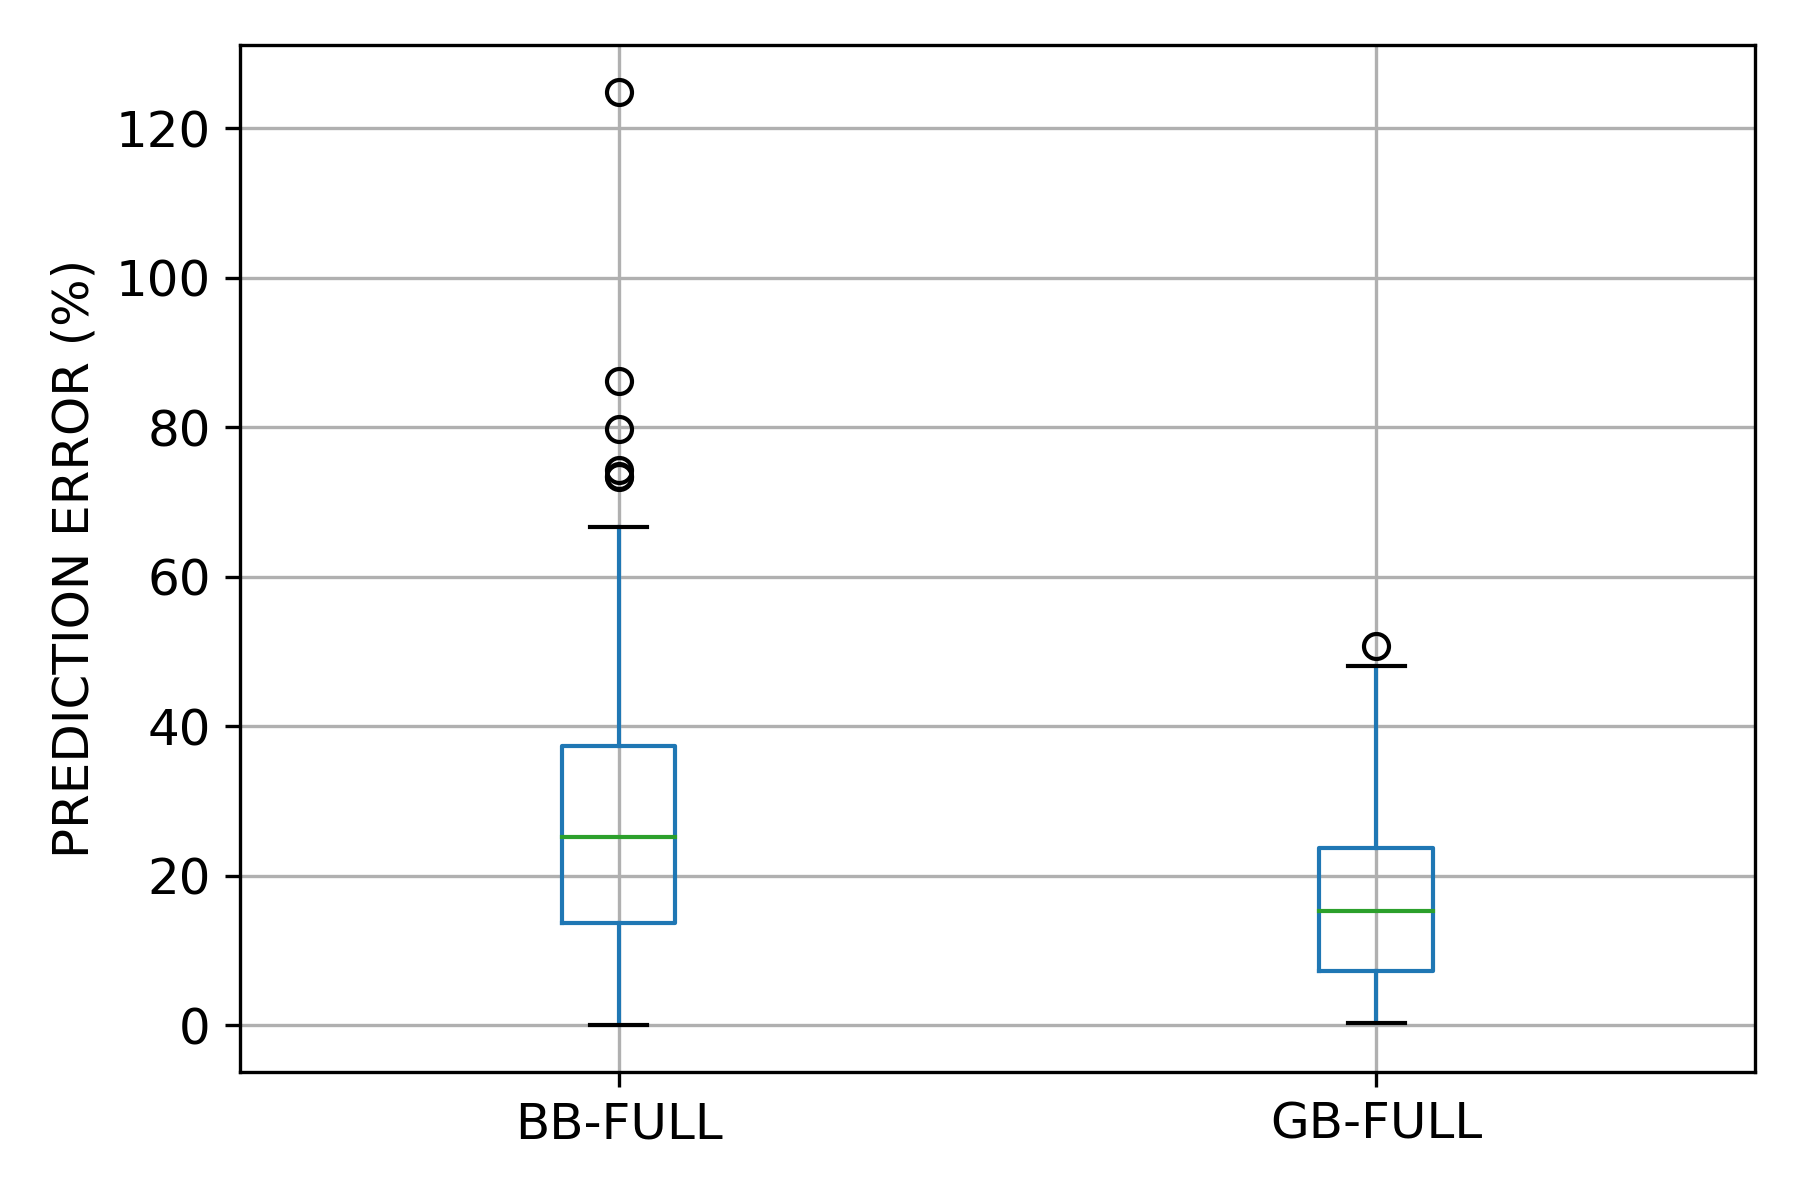
\includegraphics[width=0.37\textwidth]{sources/wexec.png}
  \caption{Workflow execution time prediction error distribution for BB-FULL and GB-FULL}
  \label{fig:workex-boxolot}
\end{figure}
In order to measure the workflow execution time prediction error we automatically generated 168 workflows  with different topologies including ScQL-Map and ScQL-Join, together with other mandatory entry/exit tasks which, for simplicity, are not discussed in this paper.  \color{black}Each ScQL workflow was mapped to a Spark Application. On average, each generated Spark application contained 23 jobs, 117 stages and more than 16K tasks per critical stage. \color{black}
%\textbf{XXX Add some more details: in how many Spark applications they map? How long were the workflow runnings? How may Spark stages were run? How many tasks within Spark stage? You need to state this also given your assumptions above XXX}
Note that those workflows have higher complexity w.r.t. to the workflows used to build the training sets, mostly containing only the task for which the ML model was going to be build.
In other words, here we demonstrate the ability of our modular approach to predict the execution time of workflows of unseen complexity, although minimal workflows were used for training the ML models.

As described in Section \ref{section:performance_prediction}, we first estimated the input profiles for all the tasks in the DAG and then predicted each task execution time using ML models that we previously built.
We compared the workflow execution time prediction error (MAPE) for BB-FULL, i.e. the state of the art Ernest approach, and GB-FULL feature sets. The error distribution is depicted in Fig. \ref{fig:workex-boxolot}. While using BB-FULL we observed an average MAPE of \textbf{28\%}, using GB-FULL features the average MAPE dropped to \textbf{17\%}.   Moreover, while with BB-FULL (Ernest)  the error variance is higher, reaching more than 120\% prediction error in one case, the highest error measured for GB-FULL is slightly higher than 50\%.
\begin{table}[t]
\centering
\caption{Output-Estimation MAPE for ScQL-Join}\label{tab:output-estimation}
 \begin{tabular}{|c|c|c|c|}
        \hline
        \textbf{Feature} & \textbf{Analytical} | \textbf{Heuristics} & \textbf{ML} \\
        \hline
        out-num-files & 0\%  & 0.004\% \\
        out-total-size & 0.2\% & 0.11\% \\
        out-interval-length & 0.005\% & 0.03\% \\\hline
\end{tabular}
\end{table}

%scientific data-driven workflow: done

% DAG execution time / Workflow execution time:done

% include section response time in  se section  3A: done
% move the related work later on: done
% move application description before: done
% Make clear what is the performance of Ernest (for us black-box full): stated that Ernest accuracy is comparable tot hte acuracy of bb composite features
% make clear that we are showing scaling of the prediction: done?
% final plots showing errors 

% extrapoolation


% stress that workflow execution is all validation
% training on basic queries we are able to predict completely different queries (more complex / composition of basic) - external - at the end of the introduction (training and validation on totally different queries)

%

%Table with MAPE, MAP-JOIN / LOCAL-AWS
\begin{figure*}
  \centering
 \hspace*{-1cm}\begin{tabular}{ccc}
\subfloat[]{
    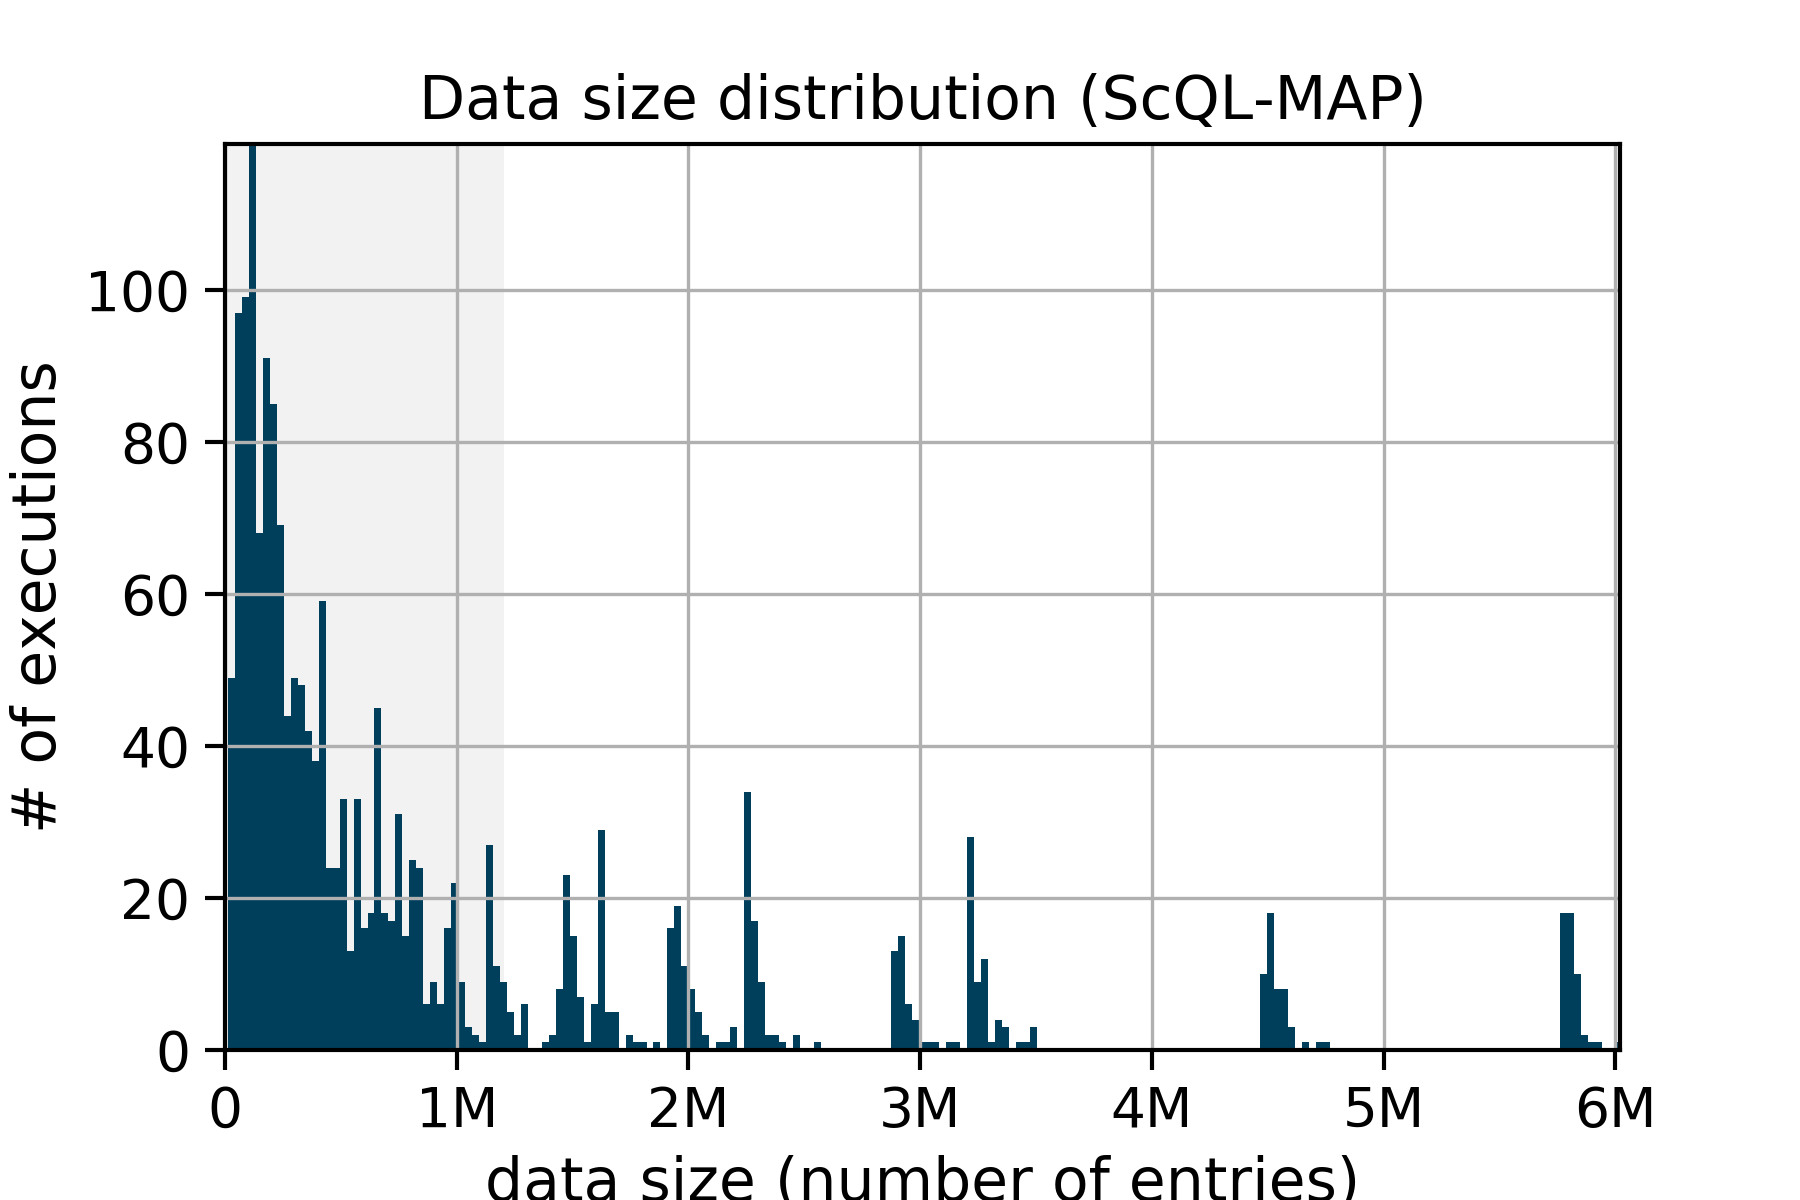
\includegraphics[width = 0.33\textwidth]{sources/Data size distribution (ScQL-MAP).png}
} &
\subfloat[]{
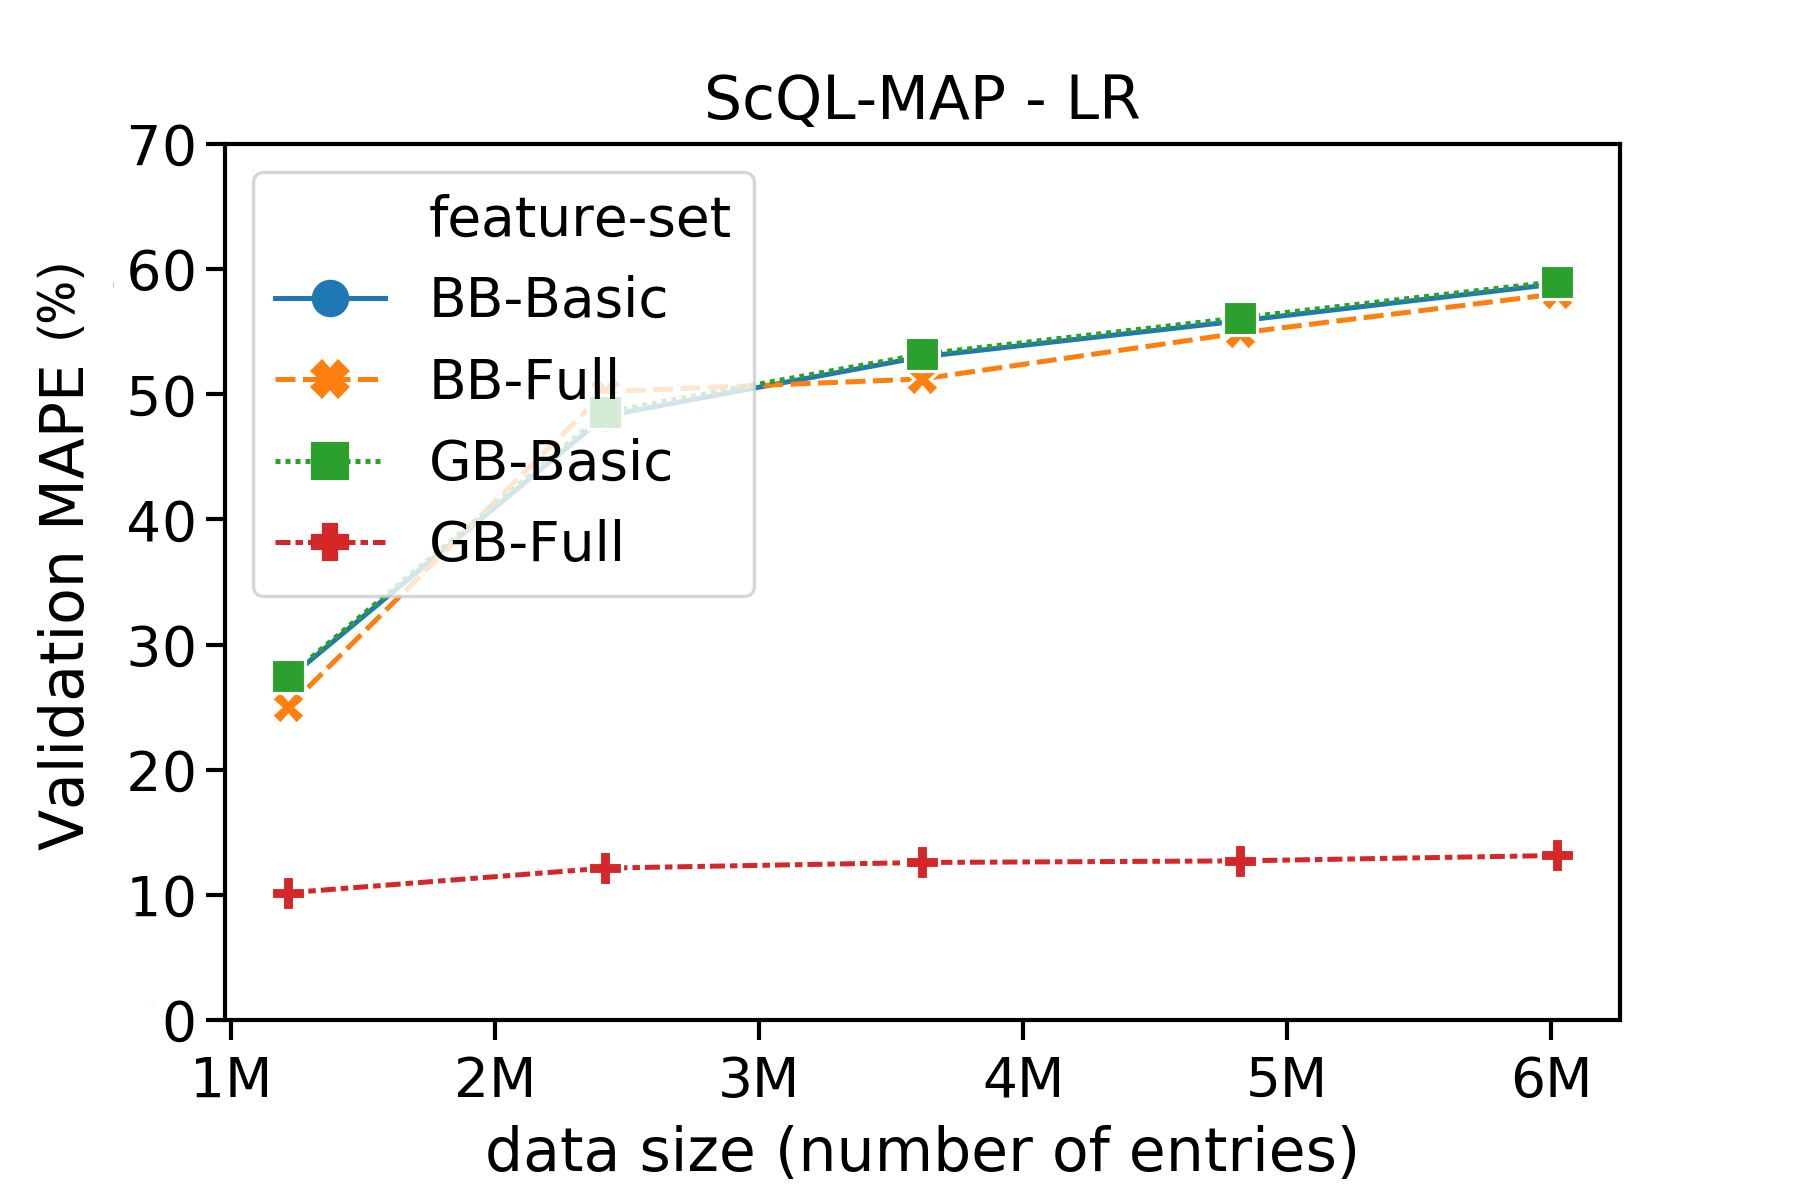
\includegraphics[width = 0.33\textwidth]{sources/ScQL-MAP - LR.png}
} &
\subfloat[]{
    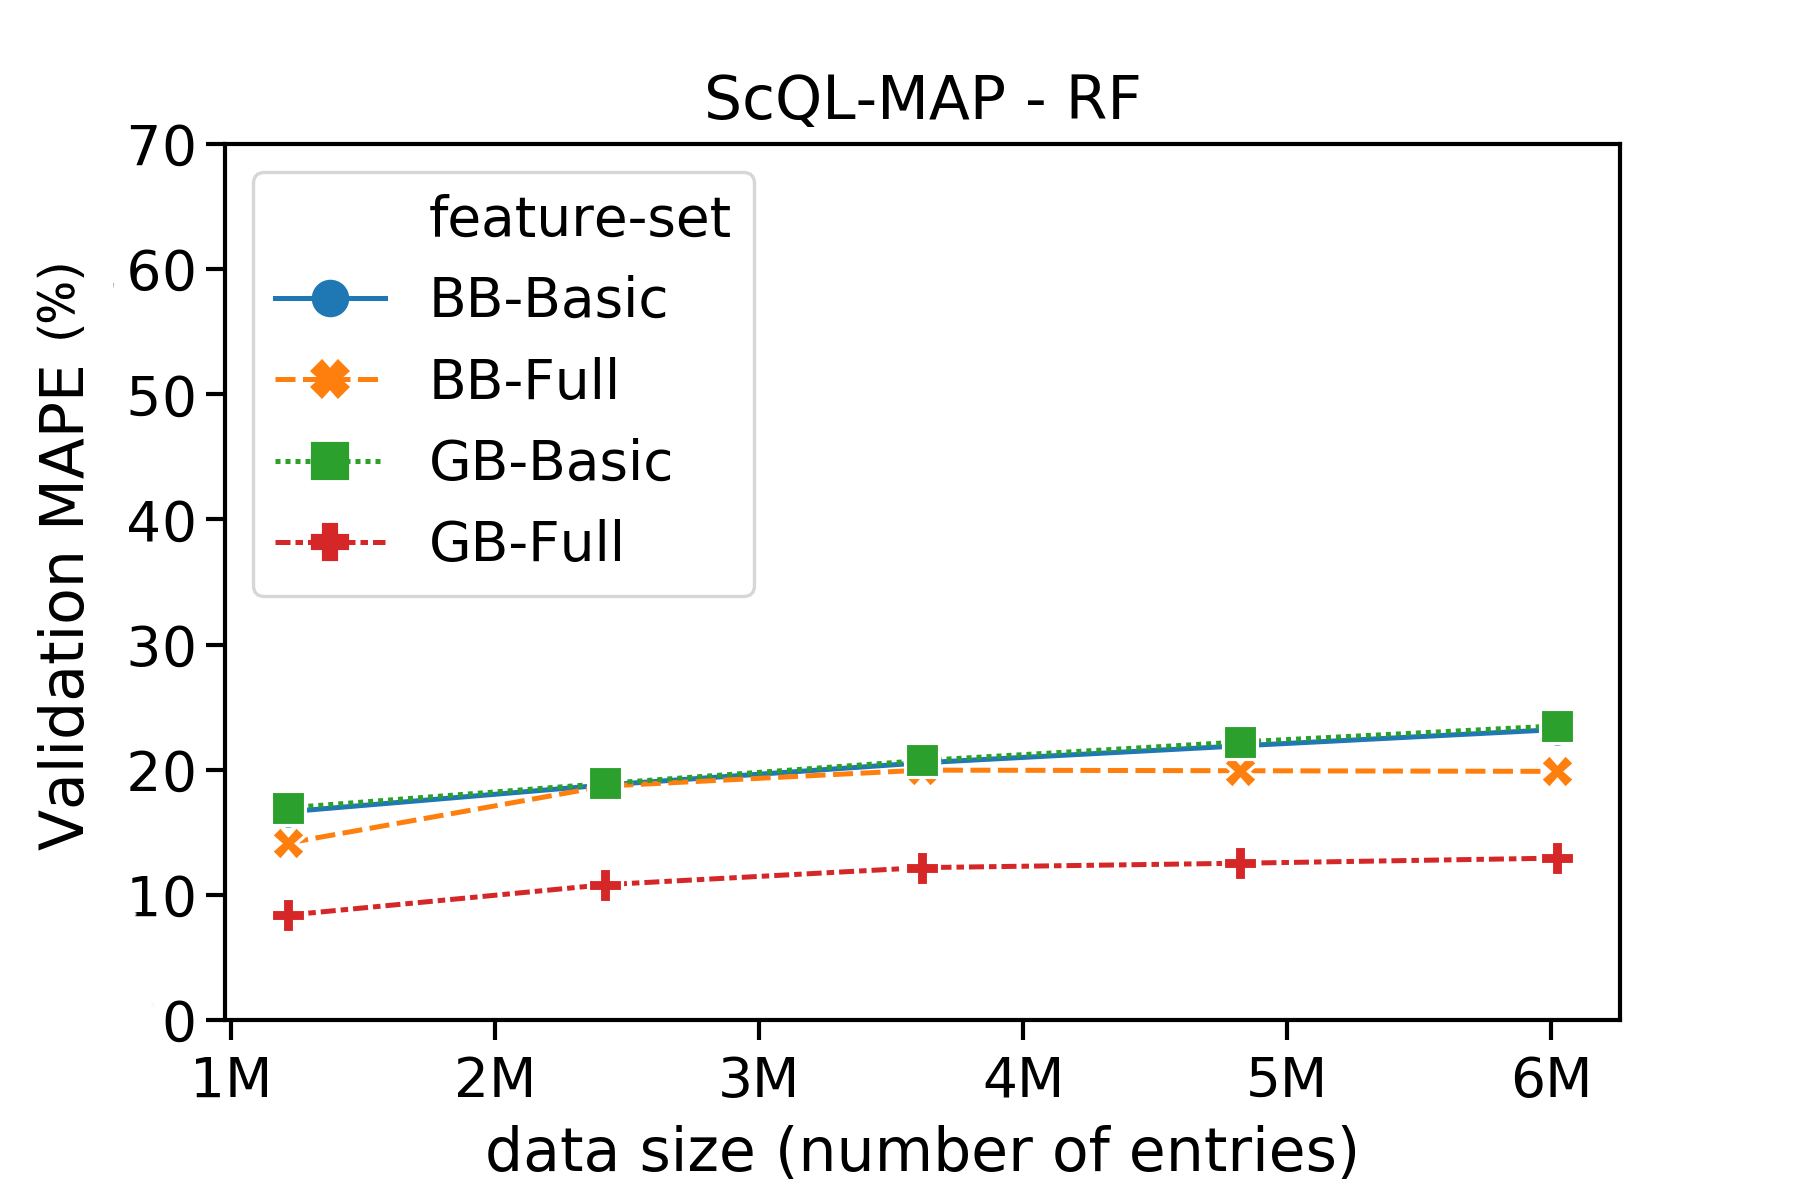
\includegraphics[width = 0.33\textwidth]{sources/ScQL-MAP - RF.png}
}  \\
\subfloat[]{
    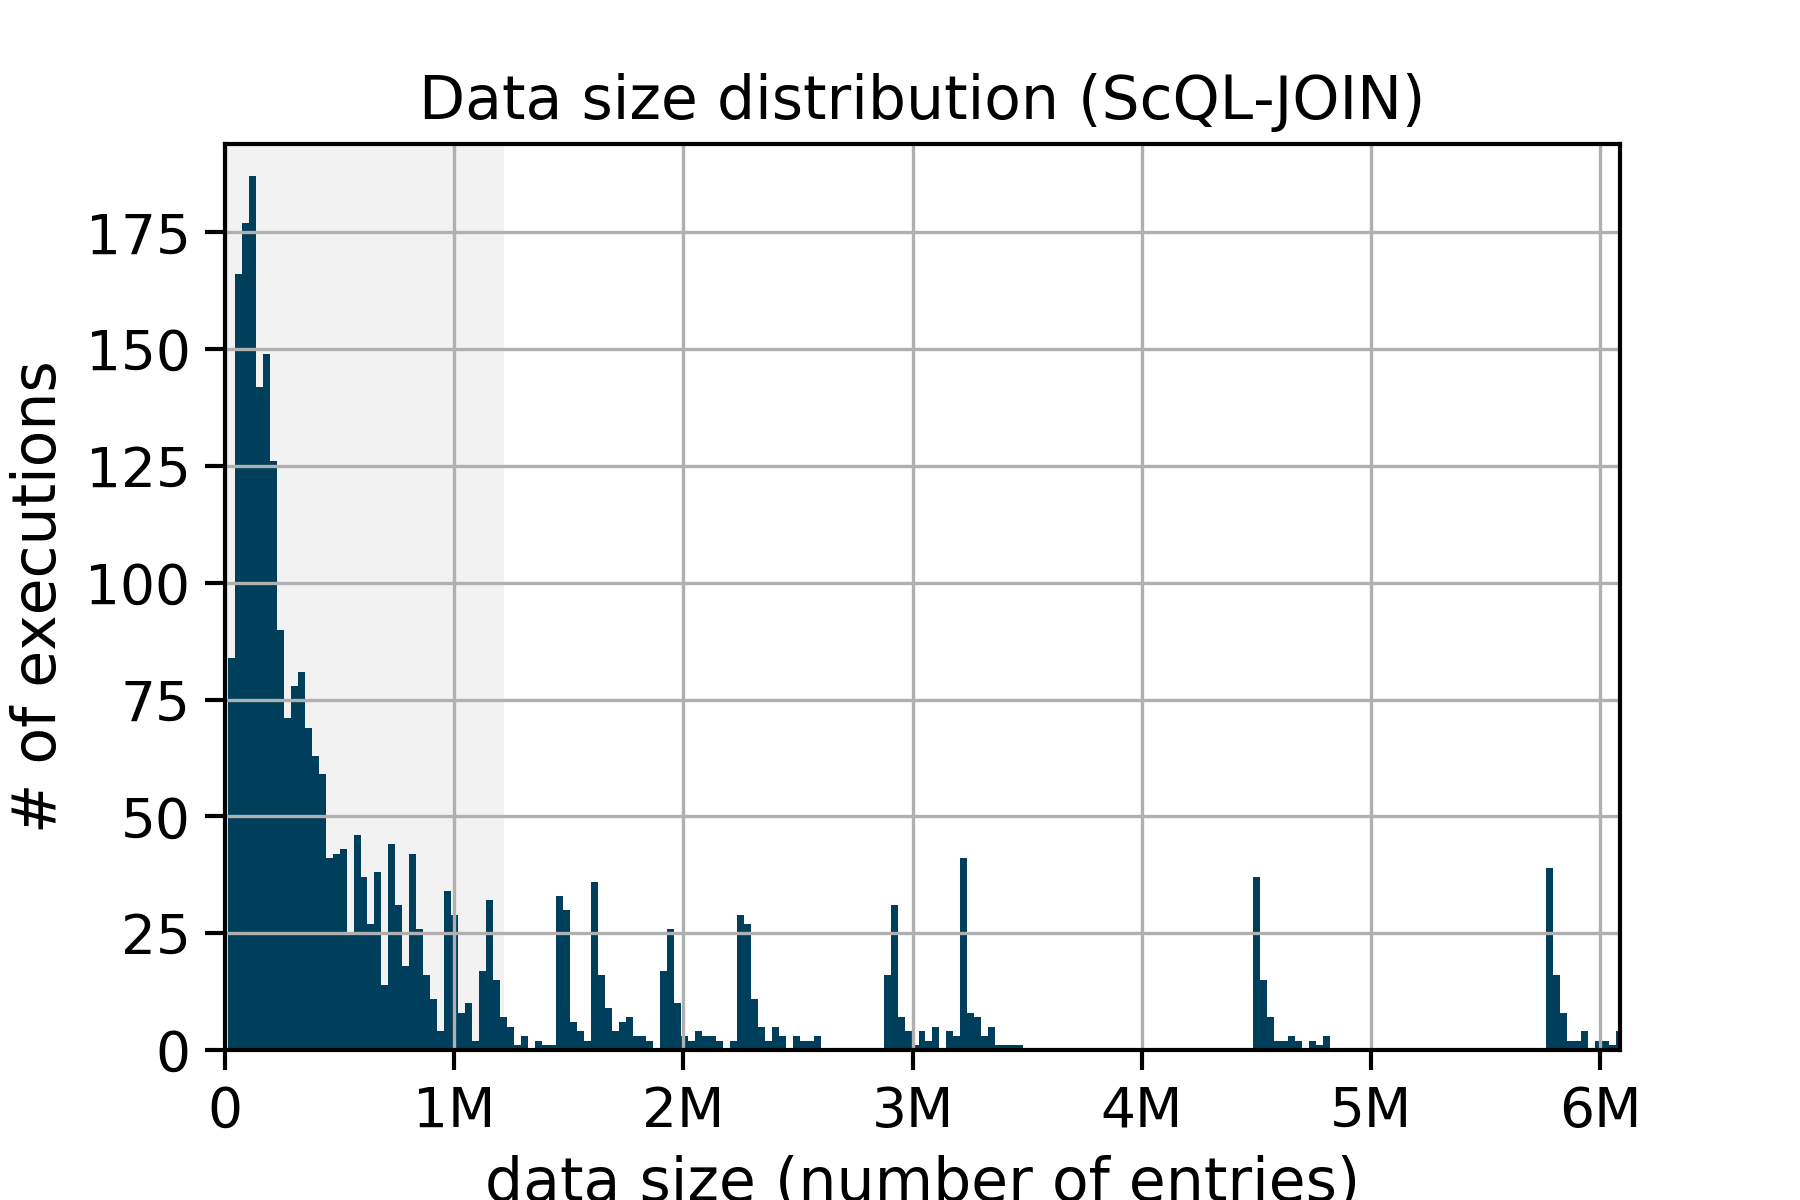
\includegraphics[width = 0.33\textwidth]{sources/Data size distribution (ScQL-JOIN).png}
}  &
\subfloat[]{
    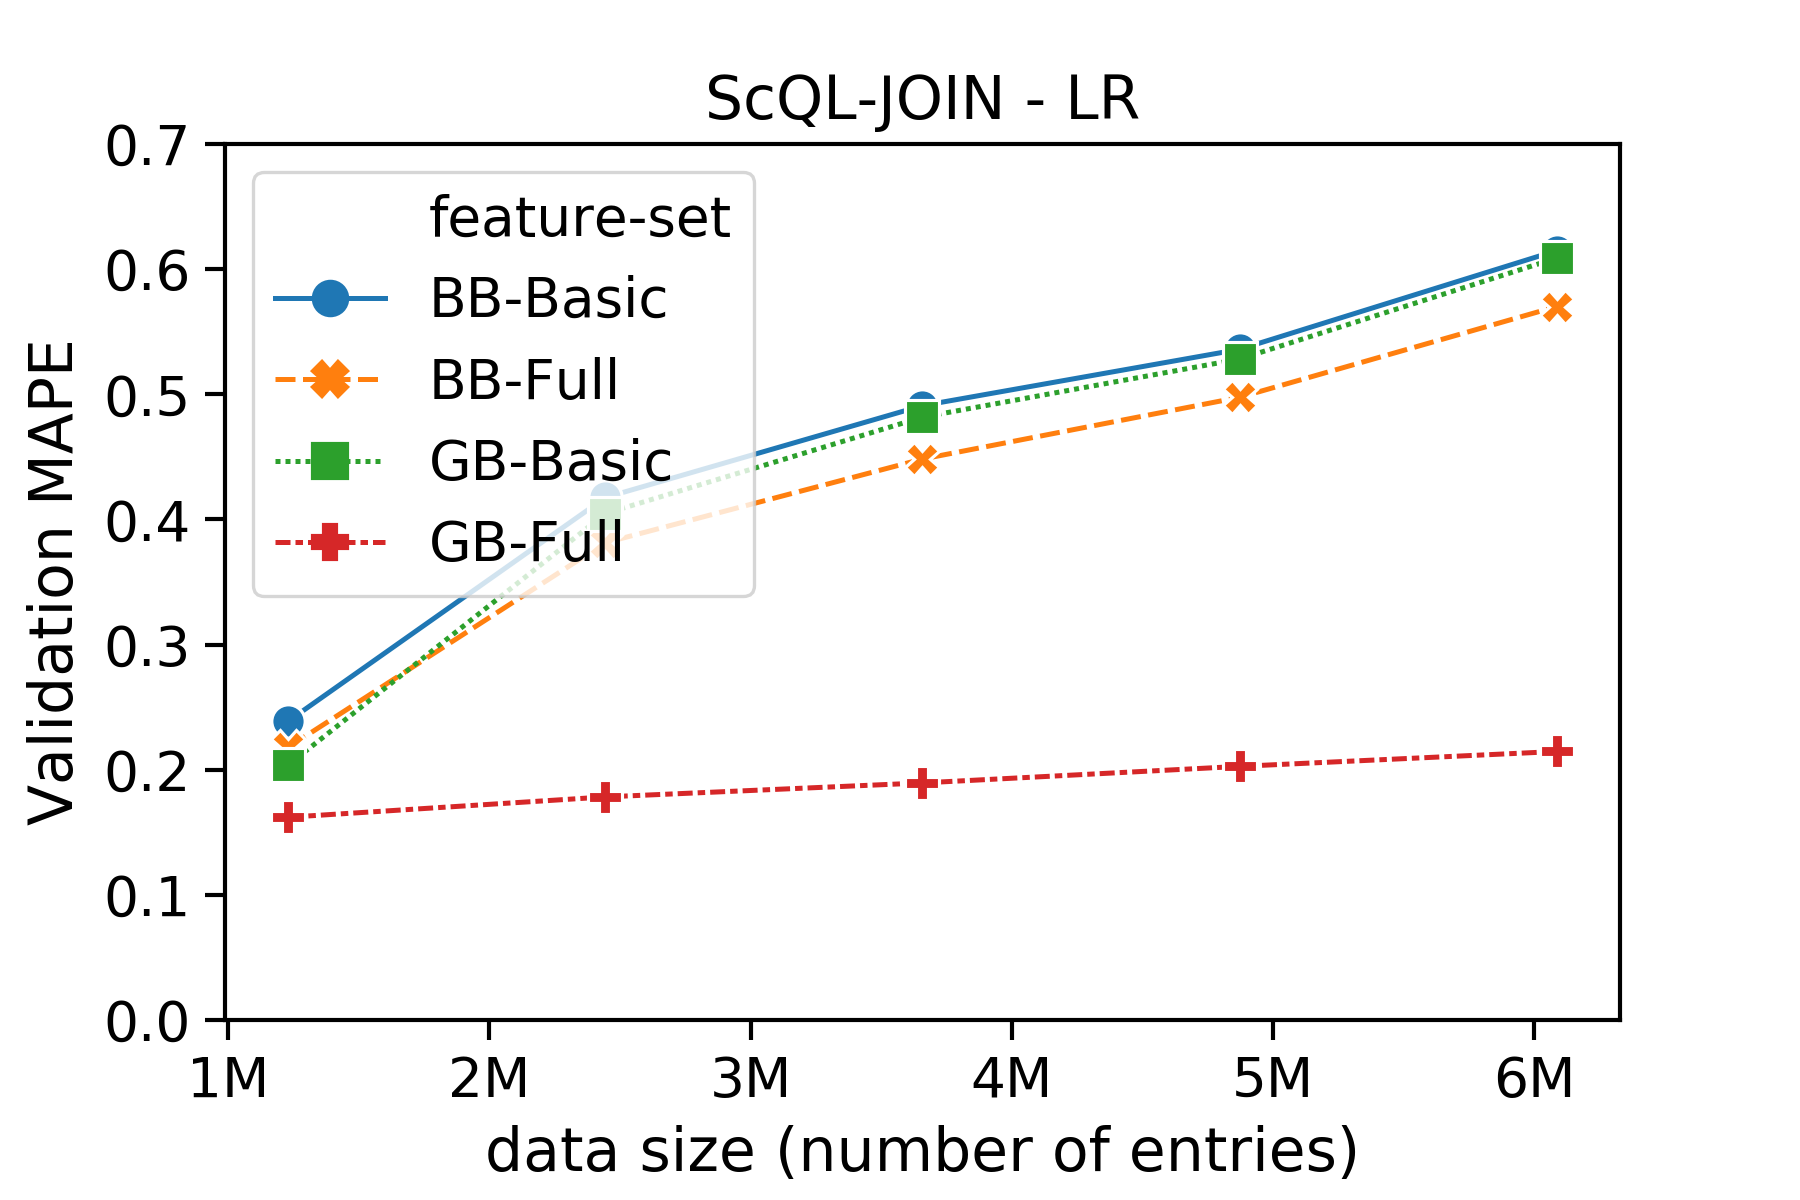
\includegraphics[width = 0.33\textwidth]{sources/ScQL-JOIN - LR.png}
} &
\subfloat[]{
    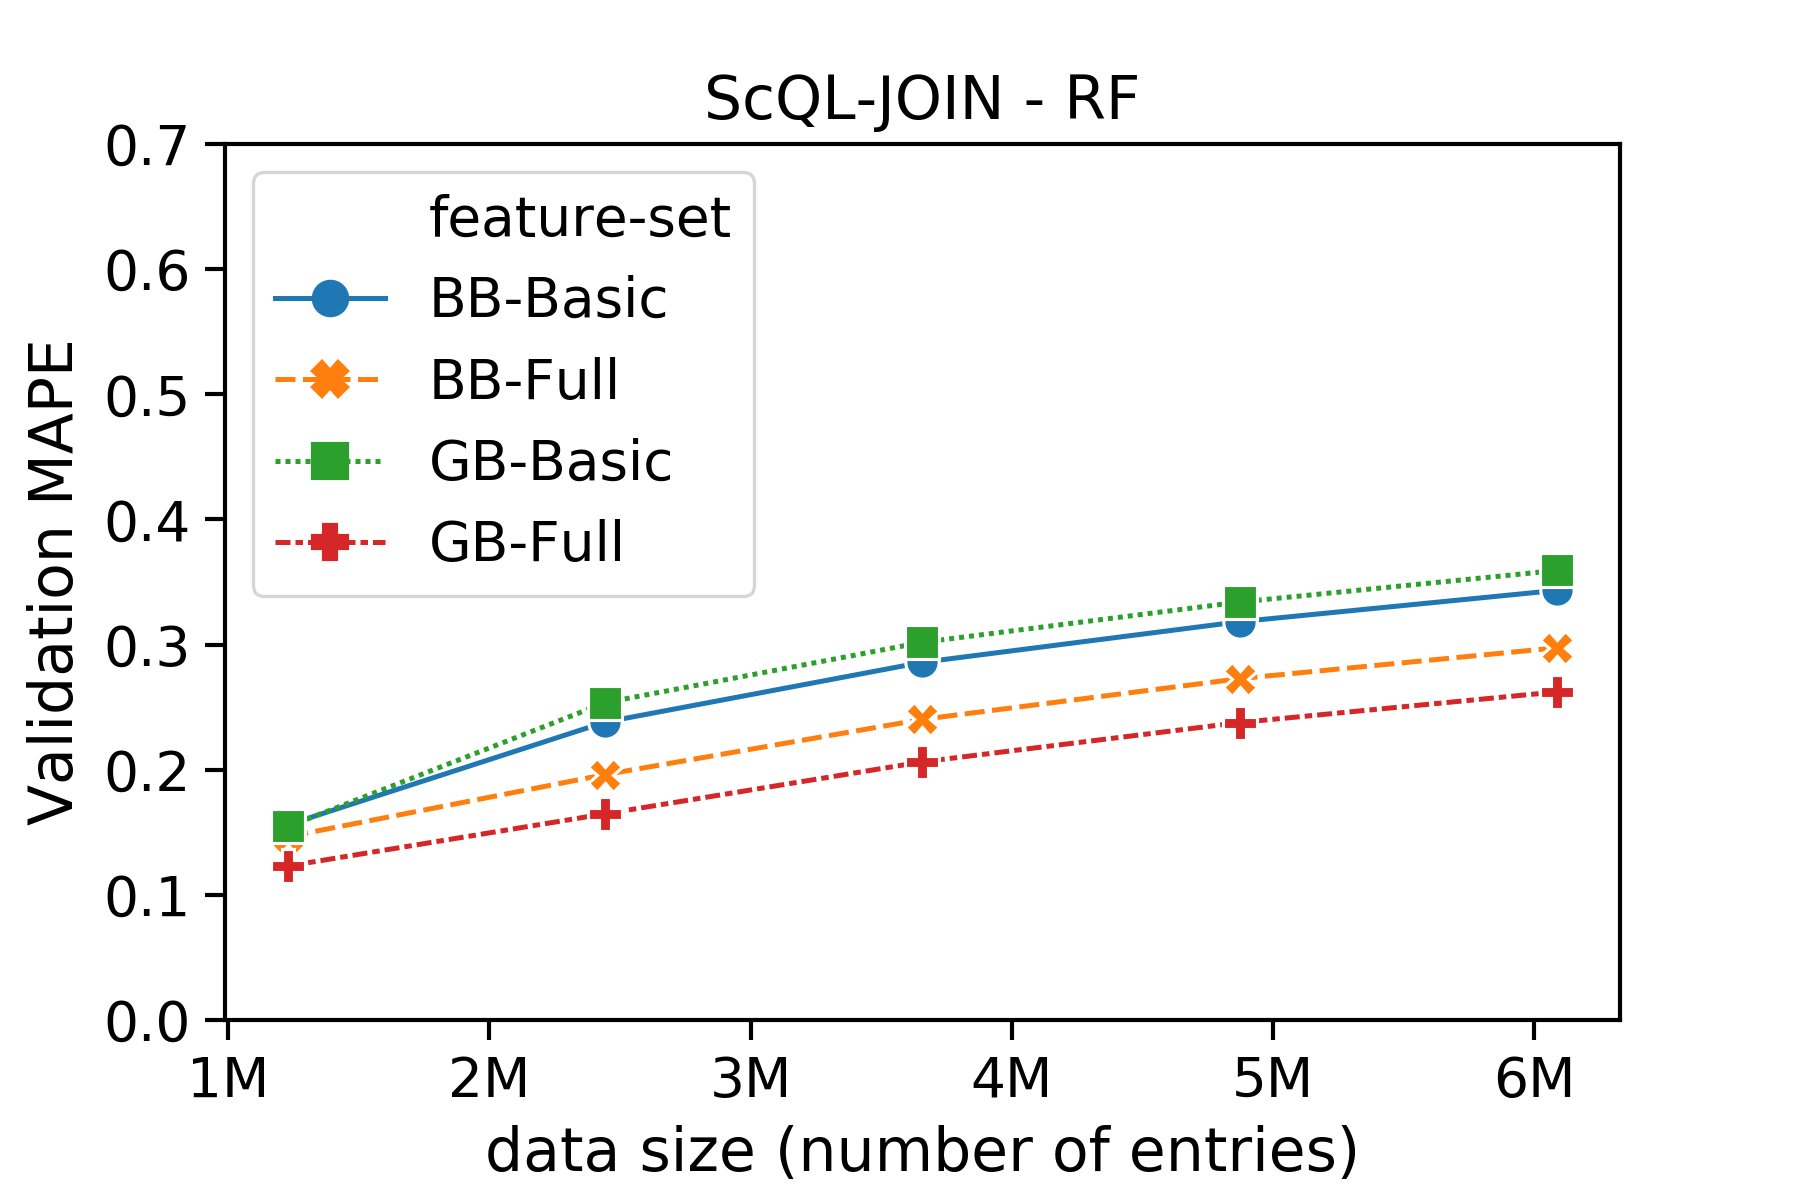
\includegraphics[width = 0.33\textwidth]{sources/ScQL-JOIN - RF.png}
} \\
\subfloat[]{
    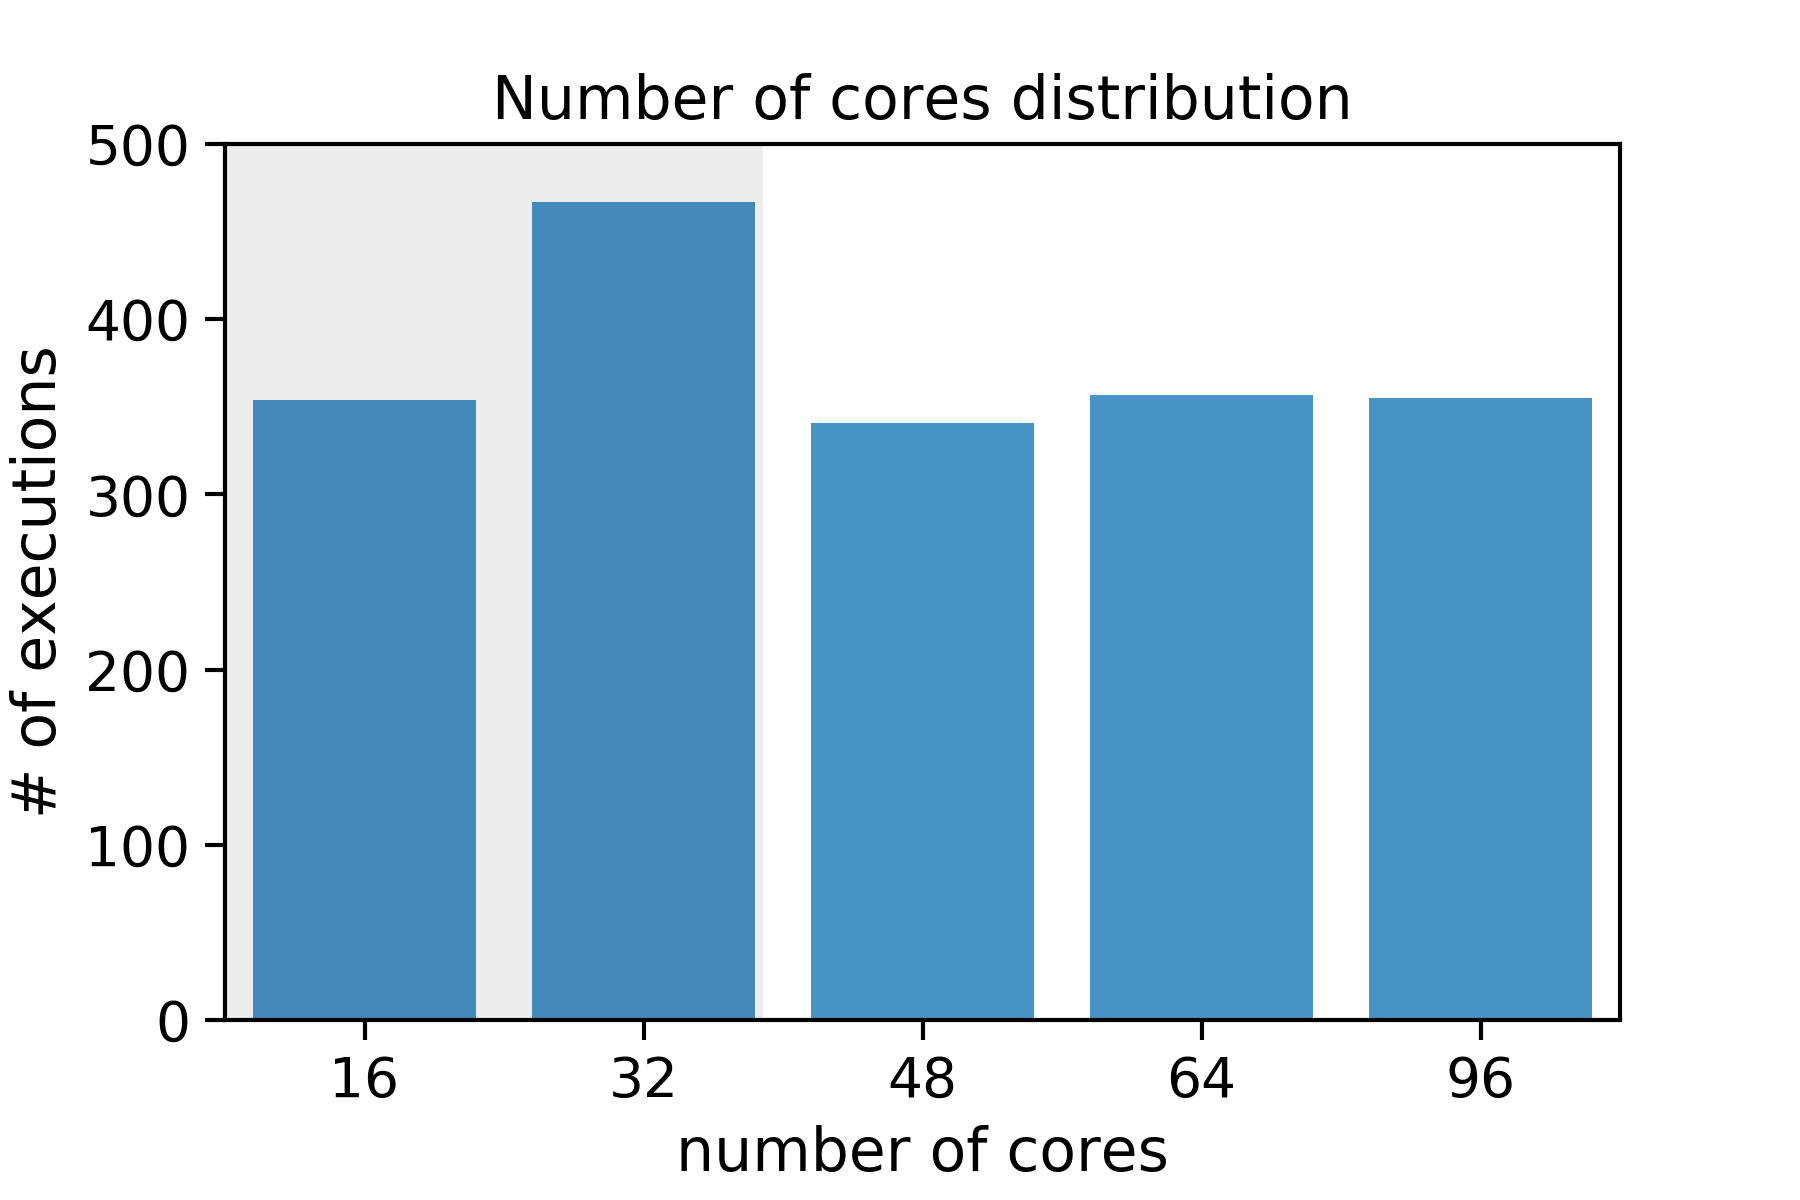
\includegraphics[width = 0.33\textwidth]{sources/cores_distribution_map.png}
}  &
\subfloat[]{
    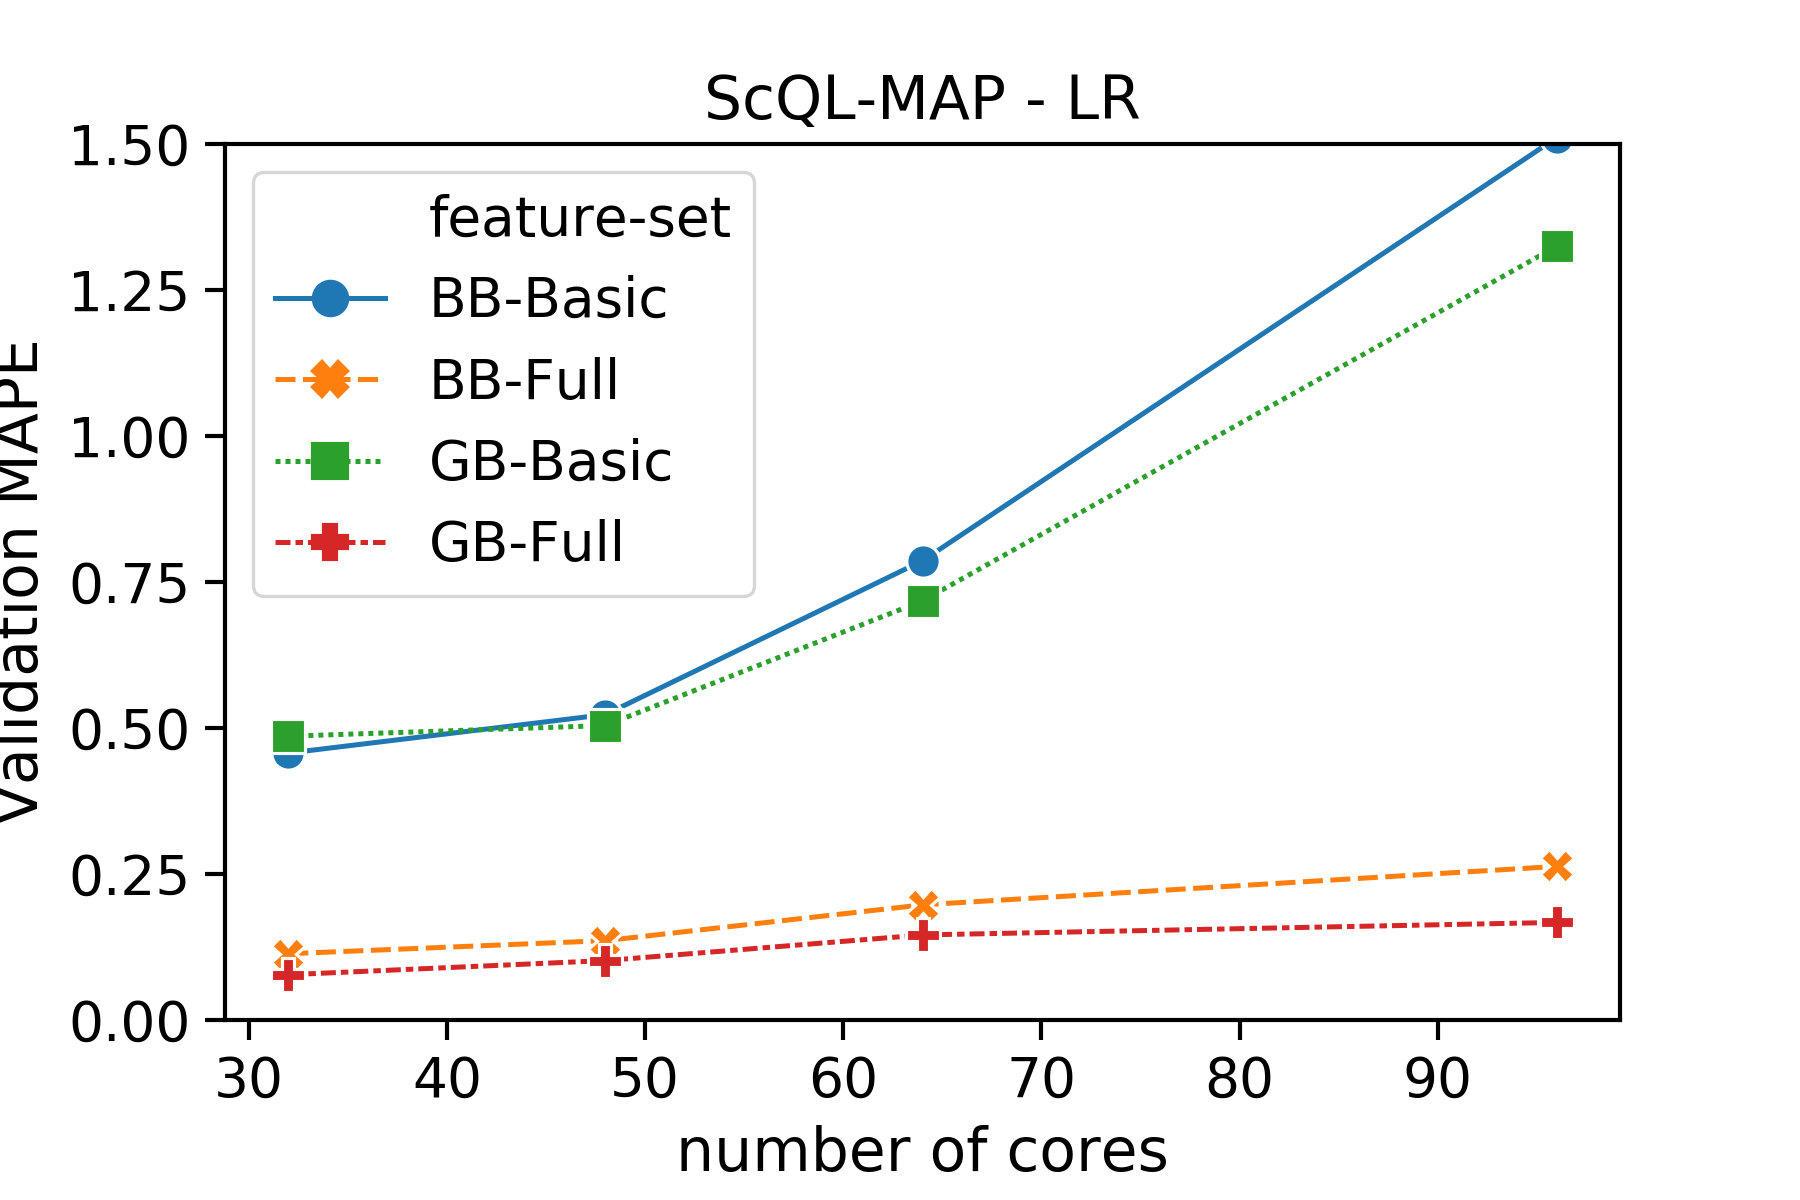
\includegraphics[width = 0.33\textwidth]{sources/ScQL-MAP - LR-cores.png}
} &
\subfloat[]{
    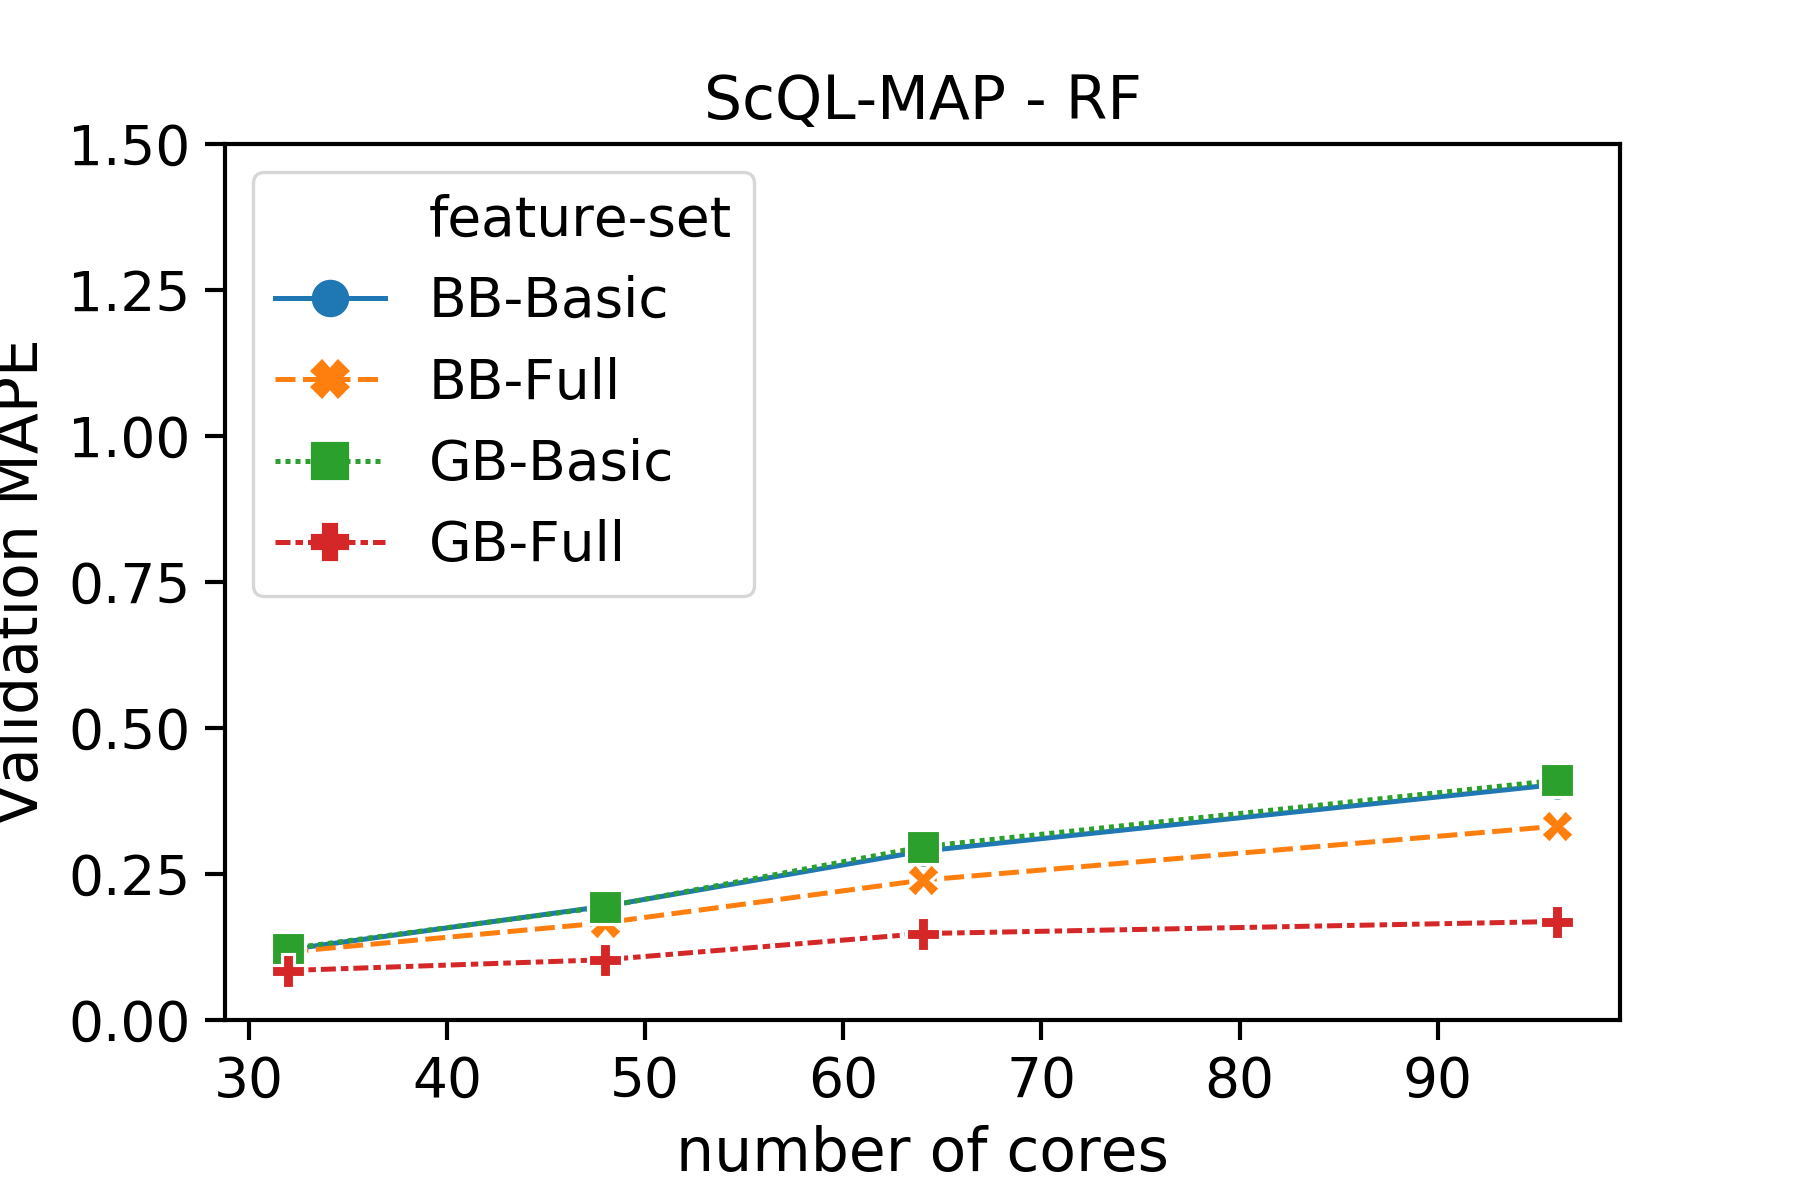
\includegraphics[width = 0.33\textwidth]{sources/ScQL-MAP - RF-cores.png}
} \\
\subfloat[]{
    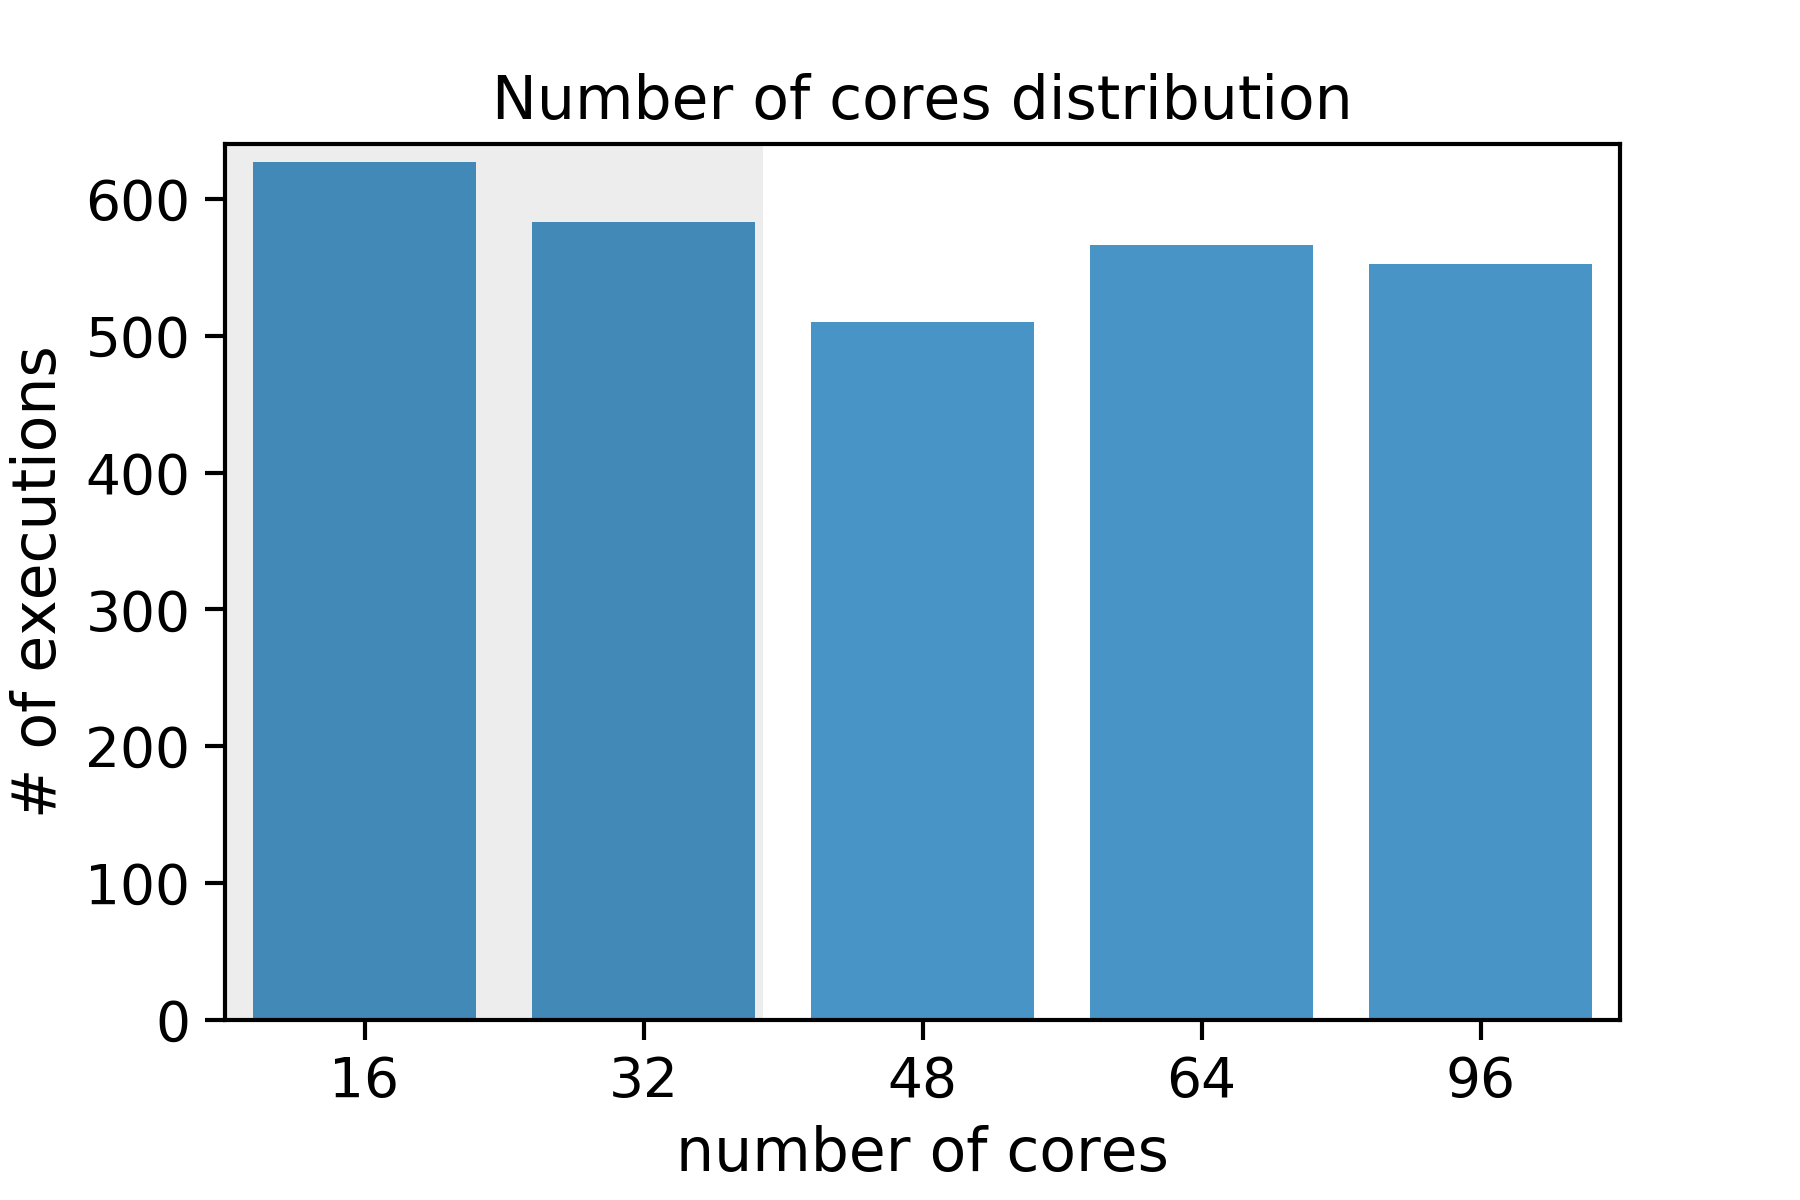
\includegraphics[width = 0.33\textwidth]{sources/cores_distribution_join.png}
}  &
\subfloat[]{
    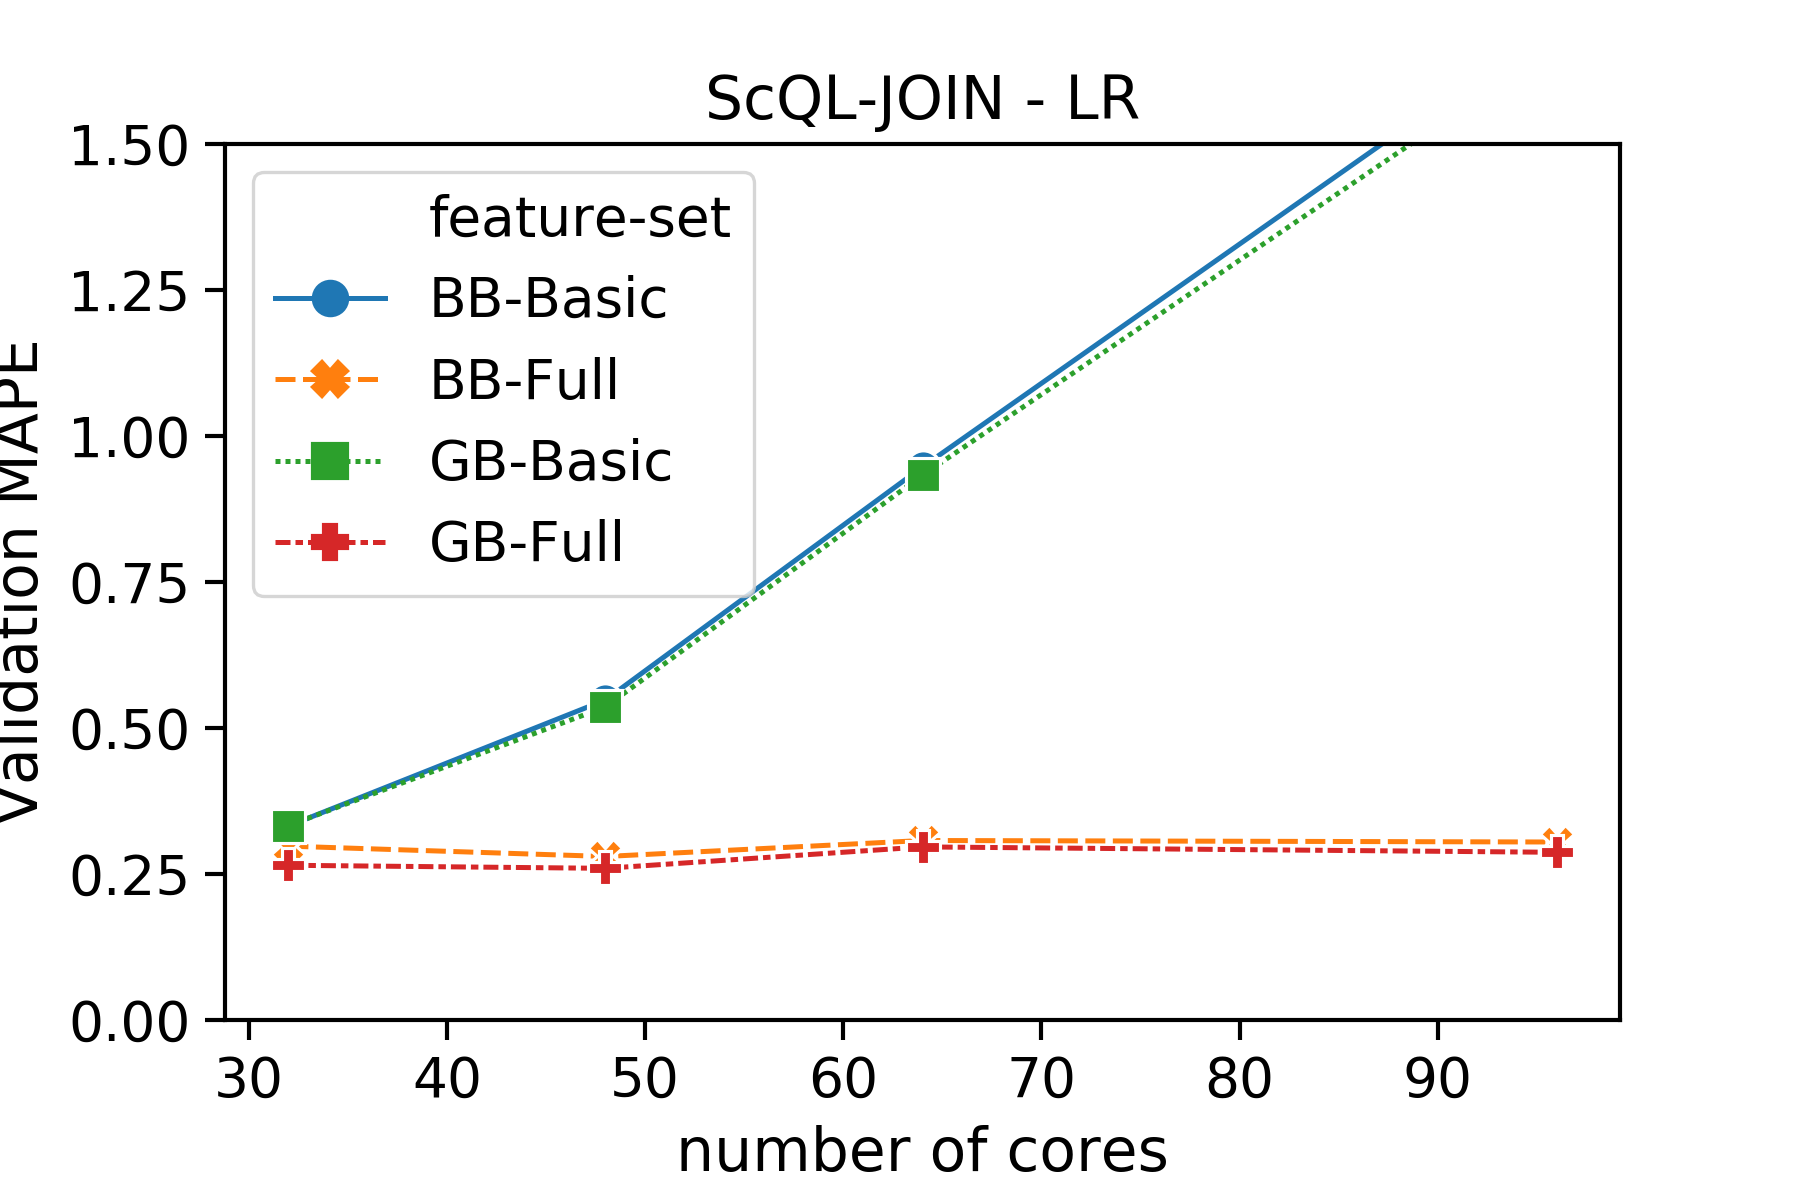
\includegraphics[width = 0.33\textwidth]{sources/ScQL-JOIN - LR-cores.png}
} &
\subfloat[]{
    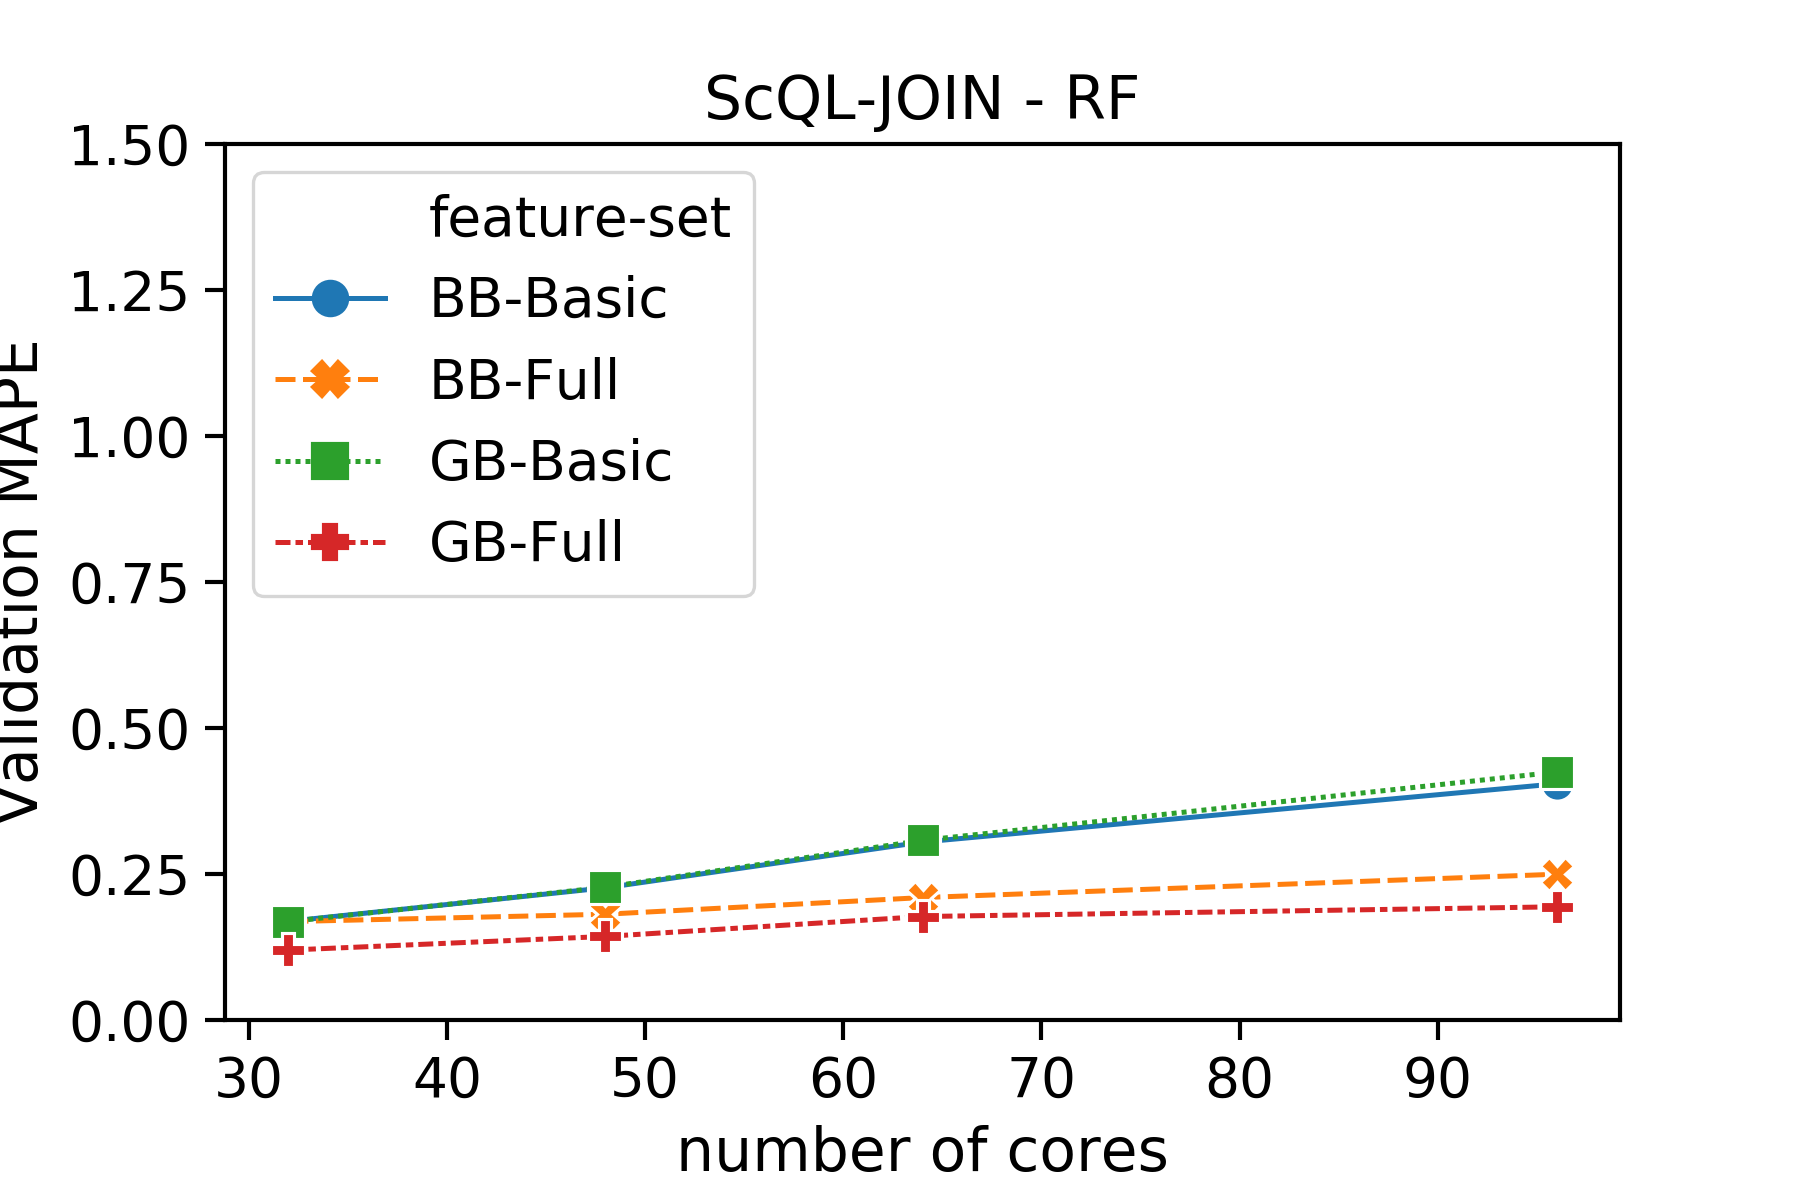
\includegraphics[width = 0.33\textwidth]{sources/ScQL-JOIN - RF-cores.png}
} 
\end{tabular}
\caption{Validation error (MAPE) variation w.r.t. the scaling of the input data size and the number of cores.}
\label{fig:scalability}
\end{figure*}



\subsection{Extrapolation analysis}
\label{subsec:extrapolation}

%\textbf{XXX The results here come from in house cluster or AWS, clarify XXX}

A desirable way to build a prediction model for performance estimation would consist in learning with small input data and few computational resources and expect a low prediction error even when the input data is much bigger and the execution environment is more powerful. In this way, the training dataset could be built in a short-time and renting expensive resources would not be necessary.
If a ML model is able to guarantee a stable prediction error for unseen value ranges of a given feature, we can say that the model is \textit{robust} against the scaling of that feature.
In this section, we compare the robustness of models, built with different  ML techniques and trained on different feature sets, w.r.t. the scaling of the number of cores and of the input data size. Since we observed that DT models are as robust as the models produced by RFs, we only show the comparison between RF and LR.\\
%\textbf{XXX Motivate why only RF and LR, most accurate? XXX: DONE, added a sentence} \\
In the first two rows of Fig. \ref{fig:scalability}, we tested the robustness against the scaling of the input data size for ScQL-MAP (first row) and ScQL-Join (second row). The first plot in each row shows on the x-axis the input data size and on the y-axis the number of executions in our dataset performed with an input of that size.
We trained the models on small executions (with input size lower than $x_0$ = 20\% of the maximum size) and measured the validation MAPE on executions belonging to unseen input size ranges: 20-40\%, 20-60\%, 20-80\% and 20-100\% of the maximum input size.
The scaling of the MAPE is depicted in the plots belonging to the second and third columns of Fig. \ref{fig:scalability}. The first point in each plot (positioned at $x_0$) represents the validation MAPE computed on some executions randomly selected  from the 0-20\% range that were not used for training. \\
Results show that RF guarantees a good scaling, while LR fails (overfits in 0-20\% range), unless gray-box full features are provided. Similarly, we tested the robustness against the scaling of the number of cores, which, for our experiments, corresponds to the scaling of the number of worker nodes in the EMR cluster. We trained our models on executions with 16 and 32 cores (i.e. 2 and 4 worker nodes), and measured the validation MAPE on executions using 48 cores, (48 \& 64) cores and (48 \& 64 \& 96) cores.\\
Again, results show that RF guarantees a good scaling, while LR fails (overfits), unless composite features are used. In this case, LR  is robust even using black-box features, given that non-linear features involving the number of cores are defined (in our feature sets  \textit{input-total-size/cores} has been selected by SFS).



\section{Related Work}
\label{section:related_work}
To the best of our knowledge, this is the first comprehensive work on performance estimation for scientific data-driven workflows, implemented on Spark, based on machine learning and analytical models. 
%Indeed, previous works have always been focused on either performance prediction for cloud-based applications (e.g. Spark Applications), or on the estimation of the workflow makespan.
Moreover, we did not find any modular workflow performance prediction solutions which explicitly address the problem of estimating intermediate tasks input data profiles, which are not known offline.
%We divide the related work in two areas i) performance prediction for Cloud-based Spark applications; ii) workflow performance prediction.  

Performance prediction for cloud-based applications has been tackled in several ways. 
Some studies apply traditional techniques, such as analytical models \cite{nelson1988approximate, mak, ardagna1, liang2000performance} and simulation \cite{bertoli2009jmt}. These techniques usually require detailed knowledge of the system, which is available only at runtime, and make  simplifying assumptions that  produce models unable to capture the complexity of cloud-based big data applications, losing in accuracy. Some studies, e.g. \cite{monotasks}, propose a change in the Spark architecture that makes the job completion time estimation easier. More recently, there have been studies exploiting machine learning (ML) models for performance prediction of large systems \cite{ernest, MUSTAFA20183767, pan2017hemingway, alipourfard2017cherrypick, ARDAGNA2019}.
Most of these works use a \textit{black-box} approach, in which historical data is used to predict future execution time, without knowledge of the system internals. Some works, instead, try to apply \textit{gray-box} approaches, taking into account some system detail \cite{ARDAGNA2019, shon2008scientific}. 
\textit{Ernest} \cite{ernest}, using simple features (functions of the input size and of the number of cores) and non-negative least squares (NNLS) regression, is considered the state-of-the-art in using ML. In \cite{ARDAGNA2019}, several ML models and several approaches (\textit{black-box} vs. \textit{gray-box}) are compared, showing better accuracy w.r.t. \textit{Ernest}.

In the area concerning workflow performance prediction, most of the works focus on the individual task execution time prediction \cite{pham2017predicting, da2015online, hilman2018task}, highlighting the important role that this prediction plays in the context of optimal workflow scheduling \cite{kousalya2017workflow}. In those papers,  machine learning techniques are applied to predict the execution time of tasks contained in different real-word static workflows, i.e. workflows with a fixed structure,  executed on the cloud. feature sets mostly accounts for environment parameters and only the workflow input data size, not the individual input to each task, is used to describe the input data.
%In \cite{pham2017predicting}, machine learning techniques are applied to predict the execution time of tasks contained in different real-word static workflows, i.e. workflows with a fixed structure,  executed on the cloud. Their feature set mostly accounts for environment parameters and only the workflow input data size, not the individual input to each task, is used to describe the input data. Similarly, in  \cite{pham2017predicting} and \cite{da2015online}, tasks runtimes, together with other parameters, are predicted for some static scientific workflows. Again, only the workflow input data size is used to build prediction models. These last works introduce an online incremental learning approach which improves estimates as more information becomes available. 

Compared to previous work, we extend performance prediction to complex Spark applications, showing the limitation of using  black-box features, and we consider complex workflows with arbitrary combinations of  tasks, whose performance can be accurately predicted thanks to intermediate output estimation.

%The workflow scheduling problem is a well-known NP-complete problem \cite{hartmanis1982computers}. However, even if there is a quite a lot of work related  to optimal scheduling, only a limited amount of work deals with performance estimation, which, however,  cannot be easily decoupled / generalized w.r.t. to the specific scheduling algorithm used by the underlying WMS (Workflow Management System).
%Most of the available estimation models deal with simple workflows having unit tasks or no dataflow latencies on homogeneus systems. Some works focus on prividing lower and upper bounds for the makespan \cite{al1990lower, jain1994lower, hu1994improved}. A level based approach partitions the DAG in levels and computes the makespan of each level, by combining / dividing the execution time of each task in a level. The makespan of all levels are summed up to produce an estimate of the overall workflow makespan.\\



\section{CONCLUSIONS}
\label{section:conclusions}
In this paper, we presented a hybrid three-phase modular solution for predicting the performance of complex data-driven workflows which can be mapped to Apache Spark applications. The workflow performance is predicted by combining individual task execution time predictions. Compared to previous works in this area, we targeted dynamic workflows, with arbitrary tasks composition, introduced intermediate-profile estimation, essential for the proposed approach, and considered a real-word complex system as a benchmark. In the experimental evaluation we compared the accuracy of different ML methods using different feature sets, which depend on how much knowledge on the application is available. Results show that, even for complex systems, performance can be predicted with good accuracy, which improves when the semantics of tasks is known, i.e. when using gray-box features. Moreover, the produced models keep a low prediction error even for \textit{unseen} input data size, amount of cluster resources and workflow dimensions.

%The modular approach proposed in this paper, which takes advantage of intermediate result estimation, is a suitable solution for task execution time prediction, independently on the Spark


\section*{ACKNOWLEDGMENT}
This work was supported by the AWS Machine Learning Research Award (MLRA) and by the Data-Driven Genomic Computing (GeCo) project, funded by the European Research Center (ERC) (Advanced ERC Grant 693174).

%\newpage
%\balance
\bibliography{b}
\bibliographystyle{IEEEtran} 


\end{document}